% Options for packages loaded elsewhere
\PassOptionsToPackage{unicode}{hyperref}
\PassOptionsToPackage{hyphens}{url}
%
\documentclass[
]{article}
\usepackage{amsmath,amssymb}
\usepackage{lmodern}
\usepackage{iftex}
\ifPDFTeX
  \usepackage[T1]{fontenc}
  \usepackage[utf8]{inputenc}
  \usepackage{textcomp} % provide euro and other symbols
\else % if luatex or xetex
  \usepackage{unicode-math}
  \defaultfontfeatures{Scale=MatchLowercase}
  \defaultfontfeatures[\rmfamily]{Ligatures=TeX,Scale=1}
\fi
% Use upquote if available, for straight quotes in verbatim environments
\IfFileExists{upquote.sty}{\usepackage{upquote}}{}
\IfFileExists{microtype.sty}{% use microtype if available
  \usepackage[]{microtype}
  \UseMicrotypeSet[protrusion]{basicmath} % disable protrusion for tt fonts
}{}
\makeatletter
\@ifundefined{KOMAClassName}{% if non-KOMA class
  \IfFileExists{parskip.sty}{%
    \usepackage{parskip}
  }{% else
    \setlength{\parindent}{0pt}
    \setlength{\parskip}{6pt plus 2pt minus 1pt}}
}{% if KOMA class
  \KOMAoptions{parskip=half}}
\makeatother
\usepackage{xcolor}
\usepackage[margin=1in]{geometry}
\usepackage{longtable,booktabs,array}
\usepackage{calc} % for calculating minipage widths
% Correct order of tables after \paragraph or \subparagraph
\usepackage{etoolbox}
\makeatletter
\patchcmd\longtable{\par}{\if@noskipsec\mbox{}\fi\par}{}{}
\makeatother
% Allow footnotes in longtable head/foot
\IfFileExists{footnotehyper.sty}{\usepackage{footnotehyper}}{\usepackage{footnote}}
\makesavenoteenv{longtable}
\usepackage{graphicx}
\makeatletter
\def\maxwidth{\ifdim\Gin@nat@width>\linewidth\linewidth\else\Gin@nat@width\fi}
\def\maxheight{\ifdim\Gin@nat@height>\textheight\textheight\else\Gin@nat@height\fi}
\makeatother
% Scale images if necessary, so that they will not overflow the page
% margins by default, and it is still possible to overwrite the defaults
% using explicit options in \includegraphics[width, height, ...]{}
\setkeys{Gin}{width=\maxwidth,height=\maxheight,keepaspectratio}
% Set default figure placement to htbp
\makeatletter
\def\fps@figure{htbp}
\makeatother
\setlength{\emergencystretch}{3em} % prevent overfull lines
\providecommand{\tightlist}{%
  \setlength{\itemsep}{0pt}\setlength{\parskip}{0pt}}
\setcounter{secnumdepth}{-\maxdimen} % remove section numbering
\linespread{2}
\usepackage{booktabs}
\usepackage{longtable}
\usepackage{array}
\usepackage{multirow}
\usepackage{wrapfig}
\usepackage{float}
\usepackage{colortbl}
\usepackage{pdflscape}
\usepackage{tabu}
\usepackage{threeparttable}
\usepackage{threeparttablex}
\usepackage[normalem]{ulem}
\usepackage{makecell}
\usepackage{xcolor}
\ifLuaTeX
  \usepackage{selnolig}  % disable illegal ligatures
\fi
\IfFileExists{bookmark.sty}{\usepackage{bookmark}}{\usepackage{hyperref}}
\IfFileExists{xurl.sty}{\usepackage{xurl}}{} % add URL line breaks if available
\urlstyle{same} % disable monospaced font for URLs
\hypersetup{
  pdftitle={Dissertation Write Up V1},
  pdfauthor={Idris Hedayat},
  hidelinks,
  pdfcreator={LaTeX via pandoc}}

\title{Dissertation Write Up V1}
\author{Idris Hedayat}
\date{}

\begin{document}
\maketitle

{
\setcounter{tocdepth}{2}
\tableofcontents
}
Planning:

Intro: - Bakgroound - Research Quesion - Introduction to statistical
methods: A Literature Review - Hierarchical Modelling - introducing r
inla packages - report structure

Introduction to data: - Data description: Domestic League Data - Data
preperation - Covariates

Exploratory Data Analysis: EDA - - - -

Model Building: Bayesian Hierarchical Modelling - - - -

Model Checking: - Model validation

Discussion: - Conclusion - Limitation - Future Work

\hypertarget{introduction}{%
\section{Introduction}\label{introduction}}

\hypertarget{background-and-motivatoin}{%
\subsection{Background and Motivatoin}\label{background-and-motivatoin}}

In 2021 many of Europe's most prominent and successful Association
Football teams engaged in discussions that led to the development of the
`European Super League' (ESL). The Super League was spearheaded by it's
12 founding members from 4 of Europe's top 5 leagues including the
biggest names in football worth billions of dollars on their own such as
Manchester United, Real Madrid, Barcelona. The competition proposed to
create a new international standard of Football with aim of providing a
more sustainable and lucrative business model for the associated clubs
as a direct competitor to the existing UEFA Champions League. The Super
League was conceptualised as a closed competition; implying that the
founding members would be guaranteed permanent membership and exemption
from relegation regardless of their performance in a season. With 20
teams in total, this would mean only the 12 founding members were
guaranteed to enjoy the expected revenues from the competition, while
the 8 others faced a constant threat of relegation. Another aim of the
league was to maintain a more competitive balance, in the sense that the
league would only contain games of the highest quality from Europe's
Best. The founders believed this would retain a larger global audience,
thus increasing the value of broadcasting rights, sponsorship and
merchandise sales. The organisers also proposed the reduction of
financial disparities with the rest of European football by proposing to
share a proportion of the revenue generated with other clubs and
investing in grassroots football development.

However, following the announcement April 18th 2021, the organizers and
teams faced vast backlash among the various stakeholders of the football
community, including fans, football governing bodies, domestic leagues,
smaller clubs, and even governments.\\
The proposed Super League marked a significant departure from the
traditional format of European Football, causing concern from European
and Global football's governing bodies; UEFA and FIFA, as well as
governments including the UK government, with prime minister at the time
Boris Johnson threatening to consider what he labelled as a
``legislative bomb'' . Critics argued the closed format would lead to
the erosion of sporting merit and integrity, many fearing the superior
ESL would damage the structure of Europe's domestic leagues, given that
the resources of the founding clubs would shift to the new competition,
devaluing the domestic leagues as a result and thus widening the
financial gap. This concentration of wealth and power was argued to
making it more difficult for smaller clubs to compete hence threatening
their long term survival. While the reader may not believe this to be of
vital concern as other matters, it must be considered that the
competition alone was expected to generate Four billion euros , and
Europe's top 5 leagues already generating billions of euros alone,
notably the Premier League with €5.492 billion. Thus there are billions
of euros at stake with the proposition of this new competition, with
many subsidiary industries such as sports betting, analytics, and
sponsorships that could be affected. So, it is of our interest to
investigate what may potentially have occurred as a result of this
possible intervention in the world of football, with Juventus,
Barcelona, and Real Madrid still yet to withdraw from the competition's
establishment, there is still a possibility for the European Super
League's fruition into reality. With the 12 founding members leaving
their respective leagues, and other clubs such as Paris Saint Germain
(Ligue 1, France) potentially leaving theirs, one might consider how
this would effect the state of the domestic league should they not
participate, who would take crown in each of the top 5 leagues?

\hypertarget{research-question}{%
\subsection{Research Question}\label{research-question}}

This project aims to explore and analyse the predicted performance of
European teams in their respective domestic leagues by modelling and
analyzing a range of factors yet to be discussed. In addition, we will
use the resulting methodology and analysis to estimate and discuss the
hypothetical outcomes in a scenario where 12 clubs have been excluded
from participating in their leagues. This exclusion will have a
significant impact on the outcome of the leagues, and in reality would
have various potential ripple effects on the teams, competitions, and
industries as a whole. By conducting a thorough analysis and exploring
the potential outcomes, we hope to provide valuable insights into the
current state of European football and the potential impact of excluding
certain clubs from participation. In doing this we hope to explore
statistical techniques that can be used to model and predict the outcome
of match results. We will look at the recent scope of literature on
statistical techniques that have been used in the prediction of match
results.

\hypertarget{introduction-to-statistical-methods-a-literature-review}{%
\subsection{Introduction to statistical methods: A Literature
Review}\label{introduction-to-statistical-methods-a-literature-review}}

\hypertarget{a-brief-history}{%
\subsubsection{A Brief History}\label{a-brief-history}}

The prediction of football match results has been of interest to
researchers and statisticians for decades. The use of binomial and
negative binomial models were explored as early as 1968 by Reep and
Benjamin in their paper ``Skill and Chance in Association Football'',
before the Poisson distribution became the prominent method of modelling
these relevant quantities. Many cite and credit Maher (1982) who
successfully demonstrated the uses of Poisson Modelling,later addressing
the relation between teams in a given match through Bivariate-Poisson
modelling. One of the most influential studies in the field came from
the work of Dixon and Coles (1997) who proposed a far more effective
Poisson Model framework. In their study they introduced further
improvements with time-weighting factors and correction terms for
low-scoring matches. Their method demonstrated improved accuracy over
previous models and has been widely reference in subsequent research.

\hypertarget{bayesian-framework}{%
\subsubsection{Bayesian framework:}\label{bayesian-framework}}

Bayesian frameworks have gained popularity over recent years due to
their ability to incorporate prior knowledge and ability to update
probabilities based on newer data, providing promising results with
their predictive capabilities. Extensions of the Bayesian framework
include the Bayesian generalised linera model of Rue and Salvesen
(2000), which has been widely referred to in subsequent research. The
framework was later improved by the promising Hierarchical Bayesian
Models of Gianluca Baio in his 2010 and 2018 papers (Baio et al.,2010)
(Baio et al., 2018). Baio's contributions have been significant to the
field of statistical methods in football match modelling. The 2010 paper
introduced a multilevel structure in their modelling to estimate
team-specific parameters nested within a mixed effects model, applied in
the context of the Italian Serie A league. They also later specified a
more complex mixture model that aimed to overcome the issue of over
shrinkage produced by the Bayesian multilevel model, in order to provide
a better fit to the data of previous season. Baio later made further
improvements to this area of the Bayesian framework in his 2018 paper
incorporating even more complex and effective mixture models accounting
for the data available at the time. His works have been widely cited in
later literature, including comprehensive reviews of Bayesian
statistical methods in football (Santos-Fernandez et al., 2019) and
studies of more modern techniques (Hubáček et al., 2019). The Bayesian
Hierarchical Model demonstrates advantages by naturally accounting for
relations between variables through the assumption that they come from a
common distribution. Overall this approach enables the effective and
comprehensive account of team performance while accounting for the
hierarchical structure of football league data. More recent research
using Bayesian frameworks include that of Razali et al (2017) exploring
the use of machine learning methods, in this case Bayesian Networks
(BNs) to model, predict, and validate match results for the English
premier League. Other recent applications have included Naive Bayes and
Tree Augmented Naive Bayes Models in Rahmanet et al.~(2018),

\hypertarget{other-methods}{%
\subsubsection{Other methods}\label{other-methods}}

Although Bayesian methods have become more prominent in the field of
predictig football results in recent years, other methods have also been
observed. In the past Bradley-Terry models (Bradey and Terry 1952) with
comparison modes pairing teams to determine the outcome of a game (Kuk
1995) have been used to estimate the probabiliies of winning, drawing,
or losing a match. Related studies in the field include Godin et al's
(2014) leveraging of contextual information via ``Twitter Microposts''
and machine learning techniques in order to comprehensively beat expert
and bookmaker predictions, a dynamic approach wit a different end goal
to the purpose of our study. Furthermore, other more relevant and modern
research cover Machine Learning Methods such as Random Forests (Groll et
al.~, 2018), Gradient Boosting and Linear Support Vector Machines,
notably by Baboota et al.~(2018) who's work has been well cited as
developments in the use of Artificial Intelligence and Machine Learning
methods continue to develop in this field.

As we can observe, the aims of the papers discussed in the literature
review vary. Some aim to simply model the outcome of the came like in
Fahrmeir and Tutz (1994) using models of paired data with time varying
features. Others investigate outcomes by predicting goals scored as seen
in Dixon and Coles 1997 and Baio et al.~(2010, 2018) while others
address other characteristics used to predict outcomes, such as passing
movements and shots per game see Reep et al (1968).

\hypertarget{introduction-to-bayesian-hierarchical-modelling}{%
\subsection{Introduction to Bayesian Hierarchical
modelling}\label{introduction-to-bayesian-hierarchical-modelling}}

For the purpose of this study regarding statistical modelling in the
prediction of football outcomes, we will be predicting outcomes of the
top five European domestic leagues utilising the Bayesian Hierarchical
Model (BHM).

(Need to expand on why?) By adding many degrees of hierarchy, BHM
enables the representation of complicated relationships and structures
within the data. This strategy is based on the Bayesian probability
theory discussed above, which offers a methodical manner to revise
beliefs or probabilities in light of new information by applying the
Bayes' theorem.

The framework used in BHM adopts a

From Bayesian Inference theory we know:

\[P(\theta ,y)=P(\theta)P(y\mid \theta)\] is the joint probability
distributions for \(\theta\) and y, written as the product of the
distributions: - the prior distribution \(P(\theta)\), which estimates
the parameter \(\theta\) before data is observed - the sampling
distribution \(P(y\mid \theta)\) , referred to as the Likelihood; the
distribution of observed data conditional on \(\theta\) .

Using Bayes Theorem:

\[P(\theta\mid y) = \frac{P(\theta,y)}{P(y)} = \frac{P(y\mid \theta)P(\theta)}{P(y)}\]
Where \(P(\theta\mid y)\) represents the posterior distribution of the
parameter \(\theta\) given observed data .\(P(y)\) reflects the marginal
likelihood, or model evidence, that is derived as the integral of the
joint probability distribution of \(\theta\) and y:

\[ P(y) = \int P(\theta)P(y\mid \theta) d\theta\] In scenarios where the
marginal likelihood is not easily obtained, one may express the
posterior distribution as:
\[P(\theta\mid y) \propto P(y\mid \theta) P(\theta) \]

Hierarchical Models:

The extension of the Bayesian framework into hierarchical modelling
incorporates two added features used in deriving the posterior
distribution: - Hyperparameters: set of parameters that are used to
determine prior distributions of other parameters uesd in the model
often referred to as lower level parameters. The hierarchical nature of
BHM allows for multiple levels, each level having its own distribution.
Parameters at the higher levels are used to determine properties of the
priors for lower-levels, which are the hyperparameters. - Hyperpriors:
these are the prior distributions on the hyperparameters, used to
express uncertainty in a hyperparameter.

The framework of the BHM: We consider the structure of a two level
Bayesian Hierarchical Model let y be a set of obesrvations
\(y_1,...,y_n\) from random variables \(Y_1,...,Y_n\) and \(\theta\) be
the set of parameters from each Y\_i; \(\theta_1,...,\theta_n\) from a
common population with distribution determined by hyperparameter
\(\phi\)

The Likelihood above is \(P(y\mid\theta,\phi)\) with \(P(\theta,\phi)\)
as its prior distribution.

\[\text{Stage 1: }y\mid\theta,\phi \sim P(y\mid\theta,\phi)\]

The prior can be expressed as
\(P(\theta,\phi) = P(\theta\mid\phi)P(\phi)\) using the definition of
conditional probability

\[\text{Stage 2: }\theta\mid\phi \sim P(\theta\mid\phi)\] The next stage
being the hyperparameter: \(\phi\) with prior distribution \(P(\phi)\) ,
referred to as the hyperprior.

\[\text{Stage 3: } \phi \sim P(\phi)\]

Using this structure we obtain the posterior distribution using bayes
theorem, expressed as:
\[P(\phi,\theta\mid y)  \propto P(y \mid\theta,\phi) P(\theta,\phi) = P(y\mid\theta ) P(\theta \mid\phi ) P(\phi)\]
Using this we can obtain probabilities from the posterior distribution.

\hypertarget{the-r-inla-package}{%
\subsection{The R-INLA package:}\label{the-r-inla-package}}

In surrounding literature regarding BHM theory, various languages are
used for modelling including R, Jags, Python, Stan (Hilbe et al., 2017),
with popular related studies such as Baio et al.'s paper (2010)
addressing the use of WinBugs software. Here they used standard Markov
Chain Monte Carlo (MCMC) methods that were used to generate samples from
the posterior distribution. However this particular method requires a
large number of iterations in order to converge, which computationally
is incredibly intensive and time consuming as the number of samples
needed increases. Although MCMC methods are able to handle very complex
and dynamic models that include a large amount of parameters making it
flexible in the modelling process, for the purpose of this particular
study it raises questions as to whether it is optimal or necessary.

Instead we will consider the R-INLA package, as used in Baio et al.'s
2018 paper for football prediction modelling. The package refers to the
Integrated Nested Laplace Approximation (INLA). This method is far more
computationally efficient compared to MCMC techniques used in fitting
Bayesian Models, particularly those with latent Gaussian Structures such
as Gaussian processes and grouped random effect models. Using a
combination of analytic approximations and numerical integration with
posterior densities, the obtained posteriors can be use to get posterior
expectations and quantiles. Thus, in hope of being able to efficiently
and effectively generate many models along with their predictions for
the different leagues we will use the INLA package going forward.

\hypertarget{report-structure}{%
\subsection{Report Structure}\label{report-structure}}

In the next chapter of the report we will introduce and inspect the data
that will be used to determine the outcome of the domestic leagues. We
then go onto introduce main concepts of the model building process,
before discussing the results obtained along with any limitations and
future outlook on the research.

\hypertarget{introducing-the-data}{%
\section{Introducing the Data}\label{introducing-the-data}}

\hypertarget{fbref-datasets}{%
\subsection{Fbref Datasets}\label{fbref-datasets}}

Data of the top 5 leagues are available from a vast array of sources,
and we select Fbref because of its comprehensive and well structure
format of each league, While providing insightful information on
characteristics such as individual player statistics, and complex
measures of performance including pass progression types and expected
goals, which may be considered for more complex models. Fbref provides
the data for each league in the same format, and unlike other sources
splits the fixtures for each team into rounds, making it very useful
when predicting and updating posterior probabilities for each round as
the leagues progress in time. Fbref gives access to multiple seasons in
time for each league, which also gives rise to the possibility of using
these past seasons in the modelling process.

\hypertarget{data-description}{%
\subsection{Data Description}\label{data-description}}

The initial Fbref fixture dataframes include fixture lists of 380 games
for leagues with 20 teams; Premier Leage, La liga, Ligue 1, and Serie A,
while Bundesliga has 18 teams and thus 306 games in a season. They
provide information on ``Wk''; the round that a particular fixture
belongs to, Date, Home Team, Away Team, Score, Venue, and other
variables that were not included in the final dataframe, namely; xG,
Attendance, Referee, as these would not be able to be reproduced every
round of prediction.

\hypertarget{data-preperation}{%
\subsection{Data preperation}\label{data-preperation}}

We then clean the data handling any missing values and correcting any
inconsistencies, particularly in the case of Premier league data. There
are 38 rounds of fixtures for each team in all leagues apart from
Bundesliga where there are 34. However in some cases there are rounds
that are rescheduled thus creating double game weeks and other
conflicts, and so in the case of the Premier League the number of rounds
has been adjusted so there are 44 rounds to avoid any conflicts making
predictions more effective in the long run. We do this and other data
preparation steps using the tidyverse set of packages in r, particularly
dplyr and tibble. We first order the data in order of data, adding
ID\_game indicating the number of the specific fixture out of the 380
that are to be played. The input data is converted into long format by
duplicating the rows of each fixture for a home and away team row,
adding a binary variable Home, 1 if the team in the row of a given
fixture is Home and 0 if away. The Opponent variable was created
grouping data by ID\_game and assigning each team's opponent as
necessary. The Venue variable is adjusted instead of being the stadium
name, to the name of the team it belongs to; ``Old Trafford'' becomes
``Manchester Utd''. We then create the following variables that are to
be used in the Bayesian Hierachical modelling processing:

\begin{longtable}[]{@{}
  >{\raggedright\arraybackslash}p{(\columnwidth - 2\tabcolsep) * \real{0.5000}}
  >{\raggedright\arraybackslash}p{(\columnwidth - 2\tabcolsep) * \real{0.5000}}@{}}
\toprule()
\begin{minipage}[b]{\linewidth}\raggedright
Variable
\end{minipage} & \begin{minipage}[b]{\linewidth}\raggedright
Description
\end{minipage} \\
\midrule()
\endhead
Goal & Number of goals scored by the specific team in a given fixture
(this will be our response) \\
Points Won & Points Gained after each fixture, 3 for Win, 1 for Draw, 0
for Loss \\
Days Since Last Game & Number of days since the last fixture played by
the specific team \\
Total Points & Cumulative points acquired by each team after accounting
for the points won in the specific game \\
Points Difference & Difference in points between the 2 teams for each
fixture \\
Relative Strength & Weighted value of total points between 2 teams of
each fixture \\
Form & proportion of points won in the last 5 games, i.e x points out of
the possible 15 \\
Goals per game (Gpg)) & Amount of goals a team has scored per game \\
Goals Conceded (GC) & Amount of goals the opponent scored against a
specific team \\
Goals Conceded Per Game(GCpg) & Amount of goals the opponent scored
against a specific team per game \\
Goal Difference (GD) & Difference between the goals scored and concede
in a given game \\
Total Goals Scored (TG) & Cumulative total of goals scored in all games
played after given game \\
Total Goal Difference (TGD) & Total Goal Difference (Total Goals Scored
- Total Goals Conceded) \\
Goal Difference-Difference (TGDDiff) & Difference in the totalgoal
difffernece between the teams of a fixture \\
Rank & The league position of a team at any given game week, (1 to 20),
decided by goal difference if tied \\
Rank Difference & Difference in league position of teams for each
fixture \\
\bottomrule()
\end{longtable}

\hypertarget{exploratory-data-analysis}{%
\section{Exploratory Data Analysis}\label{exploratory-data-analysis}}

\hypertarget{section}{%
\subsection{}\label{section}}

\hypertarget{section-1}{%
\subsection{}\label{section-1}}

\hypertarget{section-2}{%
\subsection{}\label{section-2}}

\hypertarget{section-3}{%
\subsection{}\label{section-3}}

\hypertarget{section-4}{%
\subsection{}\label{section-4}}

\hypertarget{model-building}{%
\section{Model Building}\label{model-building}}

\hypertarget{baseline-model}{%
\subsection{Baseline Model}\label{baseline-model}}

Given the literature in the field of football modelling, we follow suit
assuming the number of goals scored by a team in a given fixture follows
the Poisson Distriubtion (Maher 1982, Rue and Salvesen 2000, Baio et
al.~2010).

Such a model takes the form:

\[Y_i \sim Poisson(\lambda_{1i}) \] \[X_i \sim Poisson(\lambda_{2i}) \]
where \(X_i\) and \(Y_i\) are goals scored by home and away teams
respectively in game i, and \(\lambda_{2i}\) and \(\lambda_{2i}\) are
the respective parameters that are the measures of the scoring
intensities.

In sports modelling the use of log linear random effect modells for the
parameters \(\lambda_{1i}\) and \(\lambda_{2i}\) is common (Karlis et
al.~2003). We establish a simple baselime log linear effects model:

\[log(\lambda_{1i}) = \beta_0 + \beta_1 home + att_{h_i} + def_{a_i}  \]

\[log(\lambda_{2i}) =  B_0 + att_{a_i} + def_{h_i}\] Here i=1,2,\ldots,n
where n is the number of matches played in a season, i.e.~n=380 for
Premier League, Ligue 1, La Liga, and Serie A, whereas n = 306 for
Bundesliga. Home reflects the fixed effect parameter when a team plays
at their own Venue, evidently not appearing in the Away scoring
parameter model. The `att' and `def' random effects reflect the relative
attacking and defensive capabilities of a given team. Thus for the Home
scoring Parameter, the model uses the attack effect of the home team and
the defensive effect of the away, while for the Away scoring parameter
it is modeled using the away attack effect and the home's defense.

In this model we make the assumption that the random effects of
individual teams attacking and defending effects are in an exchangeable
structure, the order in which the teams appear in the data does not have
an impact on the inferences of their individual attacking and defending
strengths. For instance the attacking strength of a team A and the
defending strength of team B are considered to be drawn from a similar
underlying distribution, regardless of the order they appear in the
dataset. The exchangeable structure helps simplify the analysis and pool
information across different teams during the season, and the assumption
implicitly applies there is some correlation between the attack strength
of a given team, and the defense of their opponent, arising since they
are in the same game drawn from a similar underlying distribution. In
doing this we imply that teams on average are similar in offensive and
defensive capabilities, and that any differences are attributed to
random variations arising from the common distribution. In our model we
assume the effects to be distributed as

\[att_i \mid \sigma_\alpha ~ Normal(0, \sigma^2_\alpha) \\ and \\ def_i \mid \sigma_\beta ~ Normal(0, \sigma^2_\beta)\]

Below is a representation of the hierarchical structure of the model at
hand:

\hypertarget{try-something-similar-to-dag-representation-that-will-show-a-hierarchical-strucutre.}{%
\subsubsection{try something similar to DAG representation that will
show a hierarchical
strucutre.}\label{try-something-similar-to-dag-representation-that-will-show-a-hierarchical-strucutre.}}

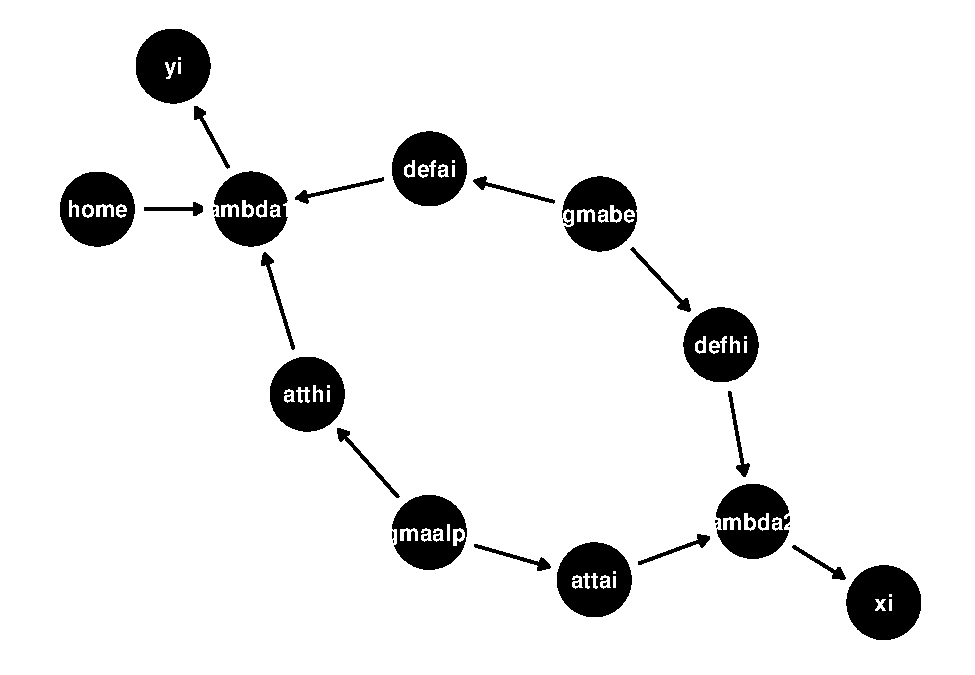
\includegraphics{DissertationWriteUpV1_files/figure-latex/DAG-1.pdf}

Having established the baseline model's formula, we fit the model using
the INLA package, again specifying the poisson distribution for he
response variable; number of Goals. Before this we prepare the data
initially on a single season for each of the leagues. We first fit the
model up to round r for prediction, with rounds 1,\ldots, r-1 having
been played already. The starting round number r was determined as the
next game week at the time of modelling, in the case of the Premier
league: 28, La Liga: 23, Ligue 1: 25, Serie A: 24, and Bundesliga: 22.

The INlA algorithm {[}Congdon, 2019{]} focuses on the posterior density
of hyperparameters \(\pi( \lambda \mid y)\) and on the conditional
posterior for the latent \(\pi(x_i \mid \lambda , y_i)\) A Laplace
approximation for marginal posterior density of random effects'
hyperparamters \(\tilde{\pi}(\lambda \mid y)\) and Taylor approximation
for conditional posterior of latent
\(\tilde{\pi}(x_i \mid \lambda , y)\) From these approximations,
marginal posteriors are obtained, where integrations are carried out
numerically.
\[\tilde{\pi}(x_i \mid y_i) = \int \tilde{\pi}(\lambda \mid y)  \tilde{\pi}(x_i \mid \lambda , y)\]
Thus, using our model the predictive distribution will have a
probability mass function {[}Baio et al., 2018{]}:

\[\tilde{\pi}(\hat{y_1} ,\hat{x_1} \mid y_1 , x_1, z_1, z_2) = \int \tilde{\pi}(\hat{y_1} ,\hat{x_1} \mid z_1 ,z_2,v)  \tilde{\pi}(v \mid y_1 , y_2,  z_1 ,z_2,)\]
Where \(\hat{y_1} ,\hat{x_1}\) are the predicted goals scored in a
future match, z\_1 z\_2 are the feature ests used, and v is the vector
of all paramaters of the model. Then cases are considered based on the
predicted goals scored:

\begin{itemize}
\tightlist
\item
  \(\hat{y_1} > \hat{x_1} \therefore\) Home Team wins
\item
  \(\hat{y_1} < \hat{x_1} \therefore\) Away Team wins
\item
  \(\hat{y_1} = \hat{x_1} \therefore\) Draw
\end{itemize}

\pagebreak

Using values from inla.summary.random we are able to extract the
quantiles of the random effects measuring the teams' attacking and
defensive strength. Below is a table showing example values of the
effects' quantiles:

\hypertarget{formatting-needed}{%
\subparagraph{Formatting needed}\label{formatting-needed}}

\begin{table}

\caption{\label{tab:unnamed-chunk-1}Example: La Liga Team Attack and Defense Random Effect Quantiles}
\centering
\resizebox{\linewidth}{!}{
\begin{tabular}[t]{c|c|c|c|c|c|c|c|c}
\hline
Team & Attack Mean & Attack 2.5\% & Attack Median & Attack 97.5\% & Defense Mean & Defense 2.5\% & Defense Median & Defense 97.5\%\\
\hline
Almería & 0.0165858 & -0.2442866 & 0.0119552 & 0.2900798 & 0.2605182 & -0.0263106 & 0.2550529 & 0.5872316\\
\hline
Athletic Club & 0.0730128 & -0.1692706 & 0.0573021 & 0.3612349 & -0.0630958 & -0.3777389 & -0.0583591 & 0.2355749\\
\hline
Atlético Madrid & 0.0678000 & -0.1751912 & 0.0528079 & 0.3537545 & -0.1970099 & -0.5575115 & -0.1861125 & 0.1066024\\
\hline
Barcelona & 0.2562312 & -0.0206139 & 0.2544078 & 0.5975623 & -0.4520438 & -0.9504112 & -0.4408945 & -0.0407376\\
\hline
Betis & 0.0325754 & -0.2204437 & 0.0240692 & 0.3083492 & -0.0609481 & -0.3755189 & -0.0563188 & 0.2380369\\
\hline
Cádiz & -0.1484229 & -0.4895383 & -0.1280458 & 0.1012194 & 0.1585272 & -0.1167629 & 0.1504560 & 0.4736459\\
\hline
Celta Vigo & -0.0430518 & -0.3291654 & -0.0326270 & 0.2173067 & 0.1492726 & -0.1269781 & 0.1411888 & 0.4639464\\
\hline
Elche & -0.1835821 & -0.5472418 & -0.1643777 & 0.0728908 & 0.3332316 & 0.0239312 & 0.3313689 & 0.6667913\\
\hline
Espanyol & 0.0109749 & -0.2509528 & 0.0076827 & 0.2823582 & 0.1419334 & -0.1359064 & 0.1338731 & 0.4568310\\
\hline
Getafe & -0.1186305 & -0.4412232 & -0.0984994 & 0.1301768 & 0.0405140 & -0.2497939 & 0.0365224 & 0.3458216\\
\hline
Girona & 0.0927870 & -0.1437525 & 0.0755216 & 0.3853525 & 0.1484430 & -0.1298679 & 0.1402905 & 0.4650535\\
\hline
Mallorca & -0.1008751 & -0.4138545 & -0.0816367 & 0.1493625 & -0.0943192 & -0.4161951 & -0.0875291 & 0.2024995\\
\hline
Osasuna & -0.1202544 & -0.4433080 & -0.1001325 & 0.1282259 & -0.1170141 & -0.4457641 & -0.1089552 & 0.1796874\\
\hline
Rayo Vallecano & 0.0329594 & -0.2199748 & 0.0243647 & 0.3088858 & -0.0417472 & -0.3506895 & -0.0387154 & 0.2577195\\
\hline
Real Madrid & 0.2835537 & -0.0125882 & 0.2857220 & 0.6354251 & -0.1912204 & -0.5519073 & -0.1802186 & 0.1130000\\
\hline
Real Sociedad & 0.0843772 & -0.1547532 & 0.0675793 & 0.3753758 & -0.0811191 & -0.4018317 & -0.0749700 & 0.2175607\\
\hline
Sevilla & -0.0262526 & -0.3049172 & -0.0198600 & 0.2377308 & 0.0701400 & -0.2138898 & 0.0642331 & 0.3768571\\
\hline
Valencia & -0.0074862 & -0.2761453 & -0.0060062 & 0.2589239 & 0.0160662 & -0.2784914 & 0.0140488 & 0.3186250\\
\hline
Valladolid & -0.1693333 & -0.5224280 & -0.1496956 & 0.0828229 & 0.0735951 & -0.2102729 & 0.0675328 & 0.3807898\\
\hline
Villarreal & -0.0319555 & -0.3119273 & -0.0242798 & 0.2300265 & -0.0941439 & -0.4161304 & -0.0873216 & 0.2025661\\
\hline
\end{tabular}}
\end{table}

Below are visual representations for the team attack and defence effects
for each of the remained of top 5 leagues, using only data from the
2022/23 seasons. We will discus later how this is impacted when adding
more data from previous seasons.

\begin{center}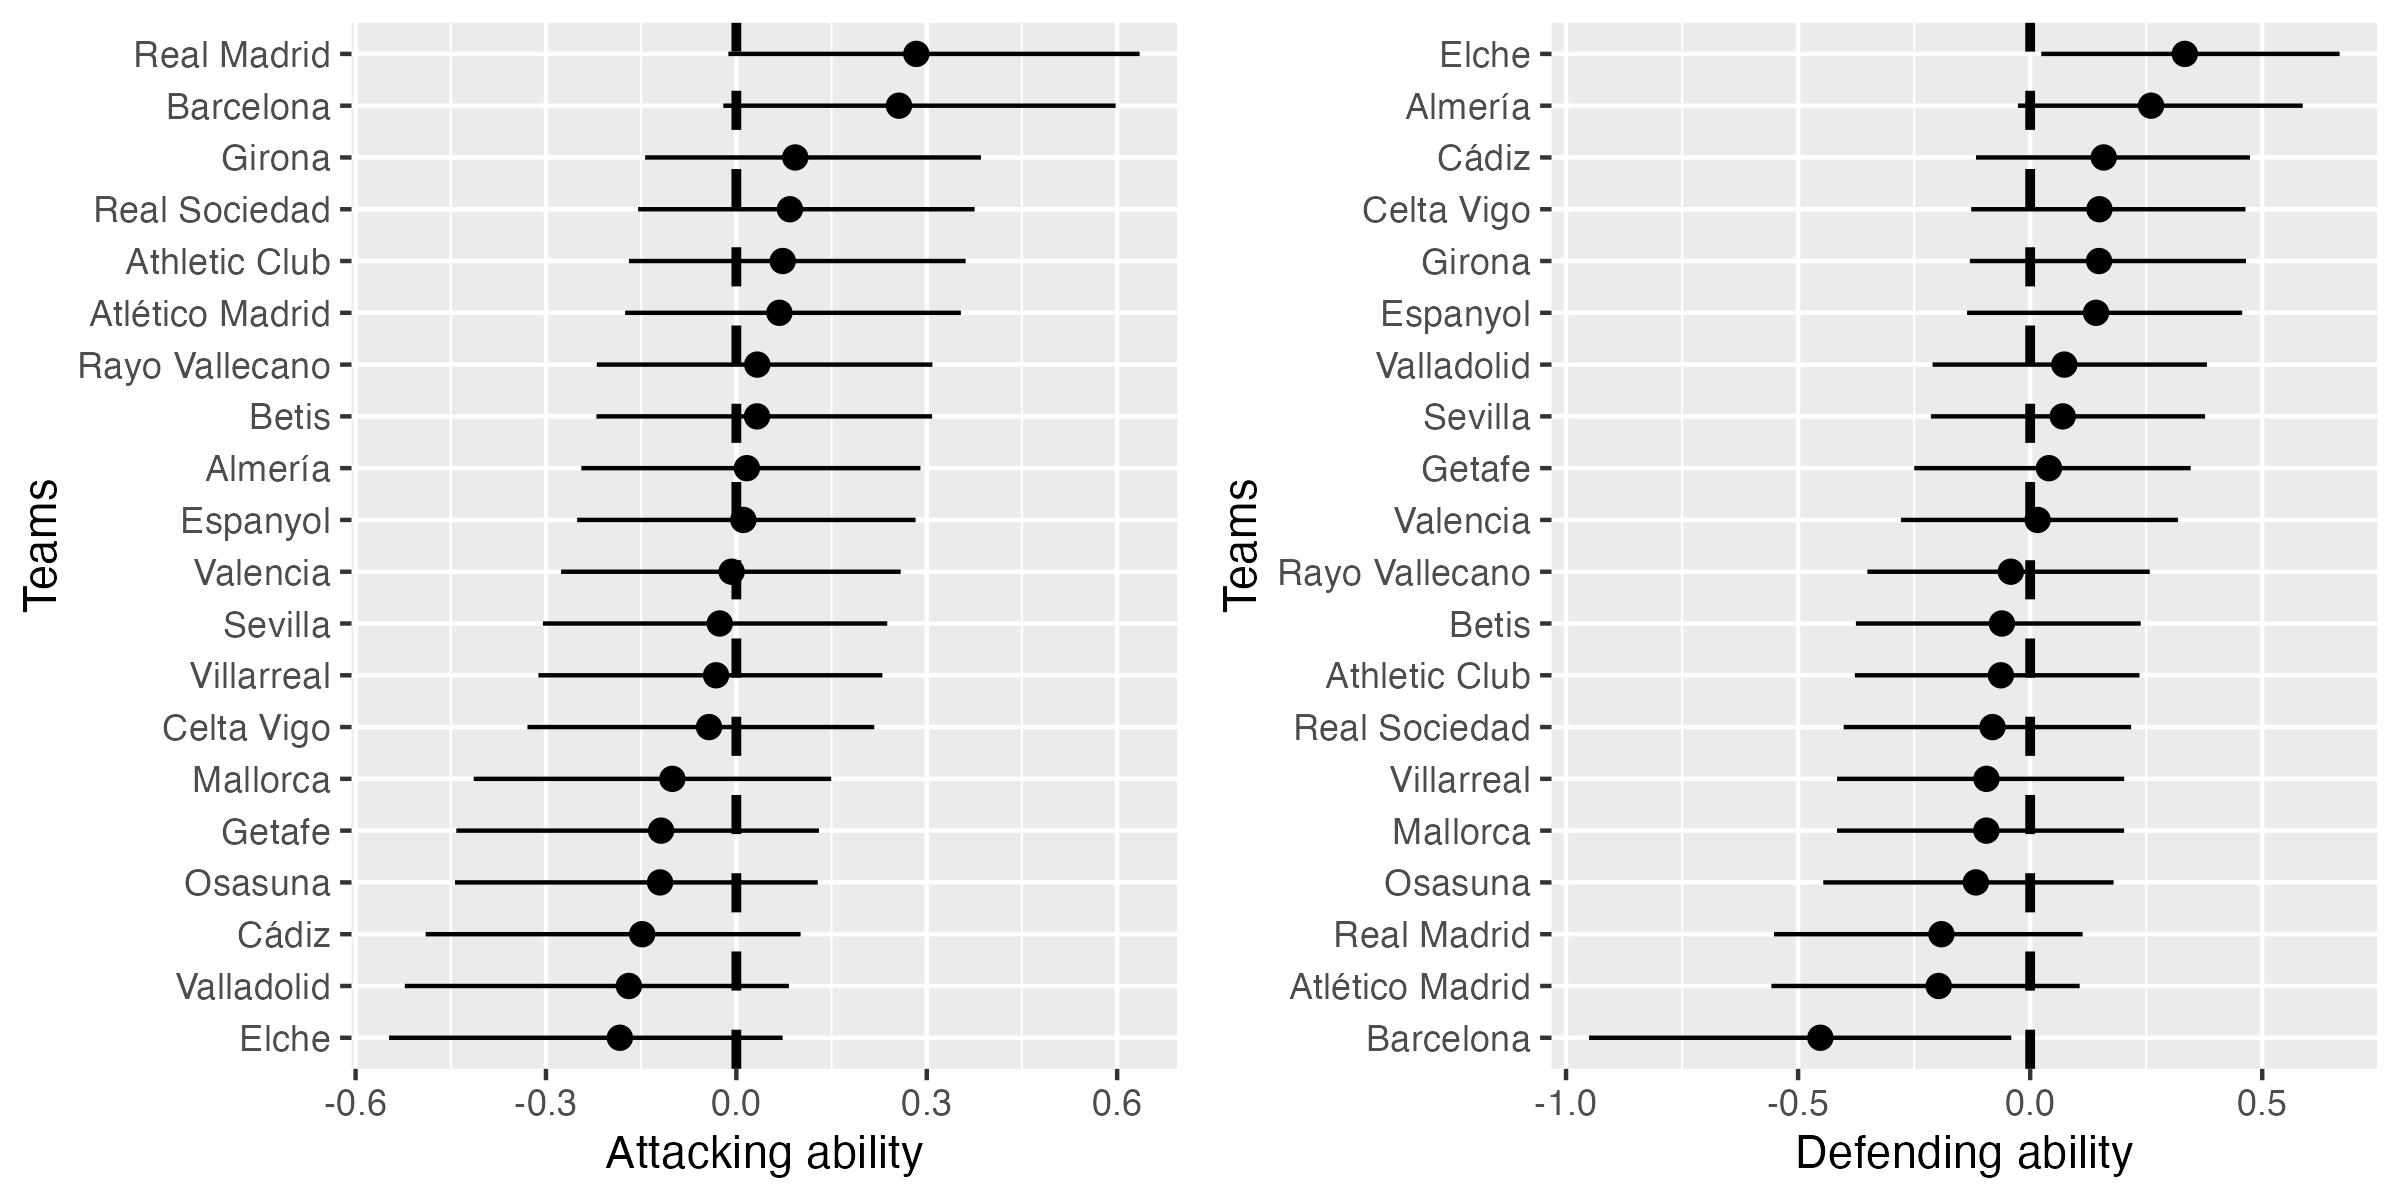
\includegraphics[width=400px]{llattdef} \end{center}

\begin{center}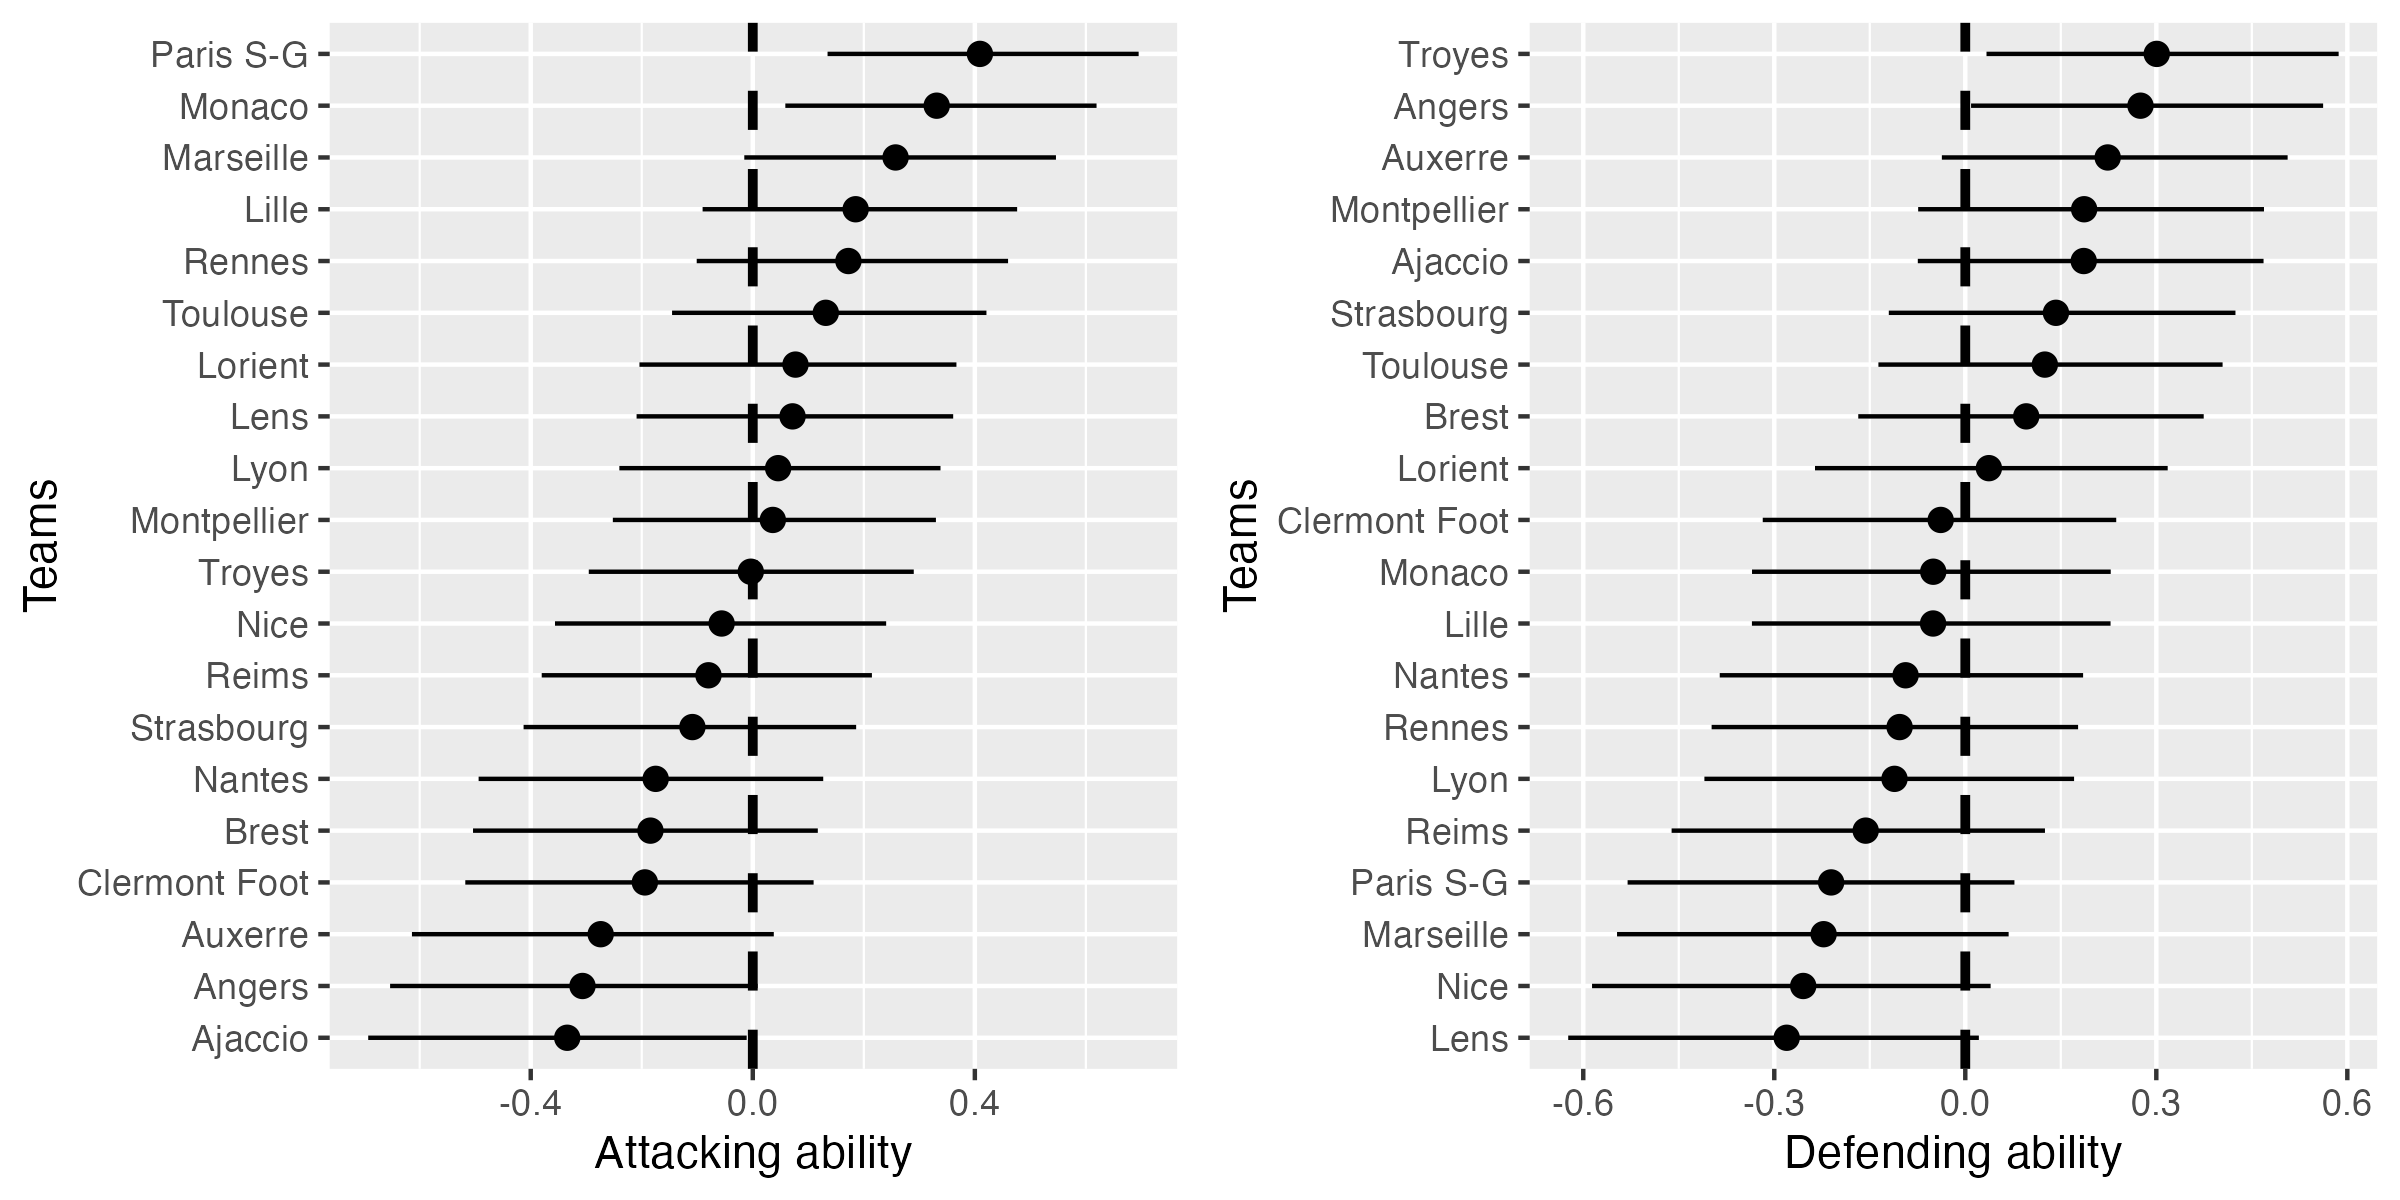
\includegraphics[width=400px]{l1attdef} \end{center}

\begin{center}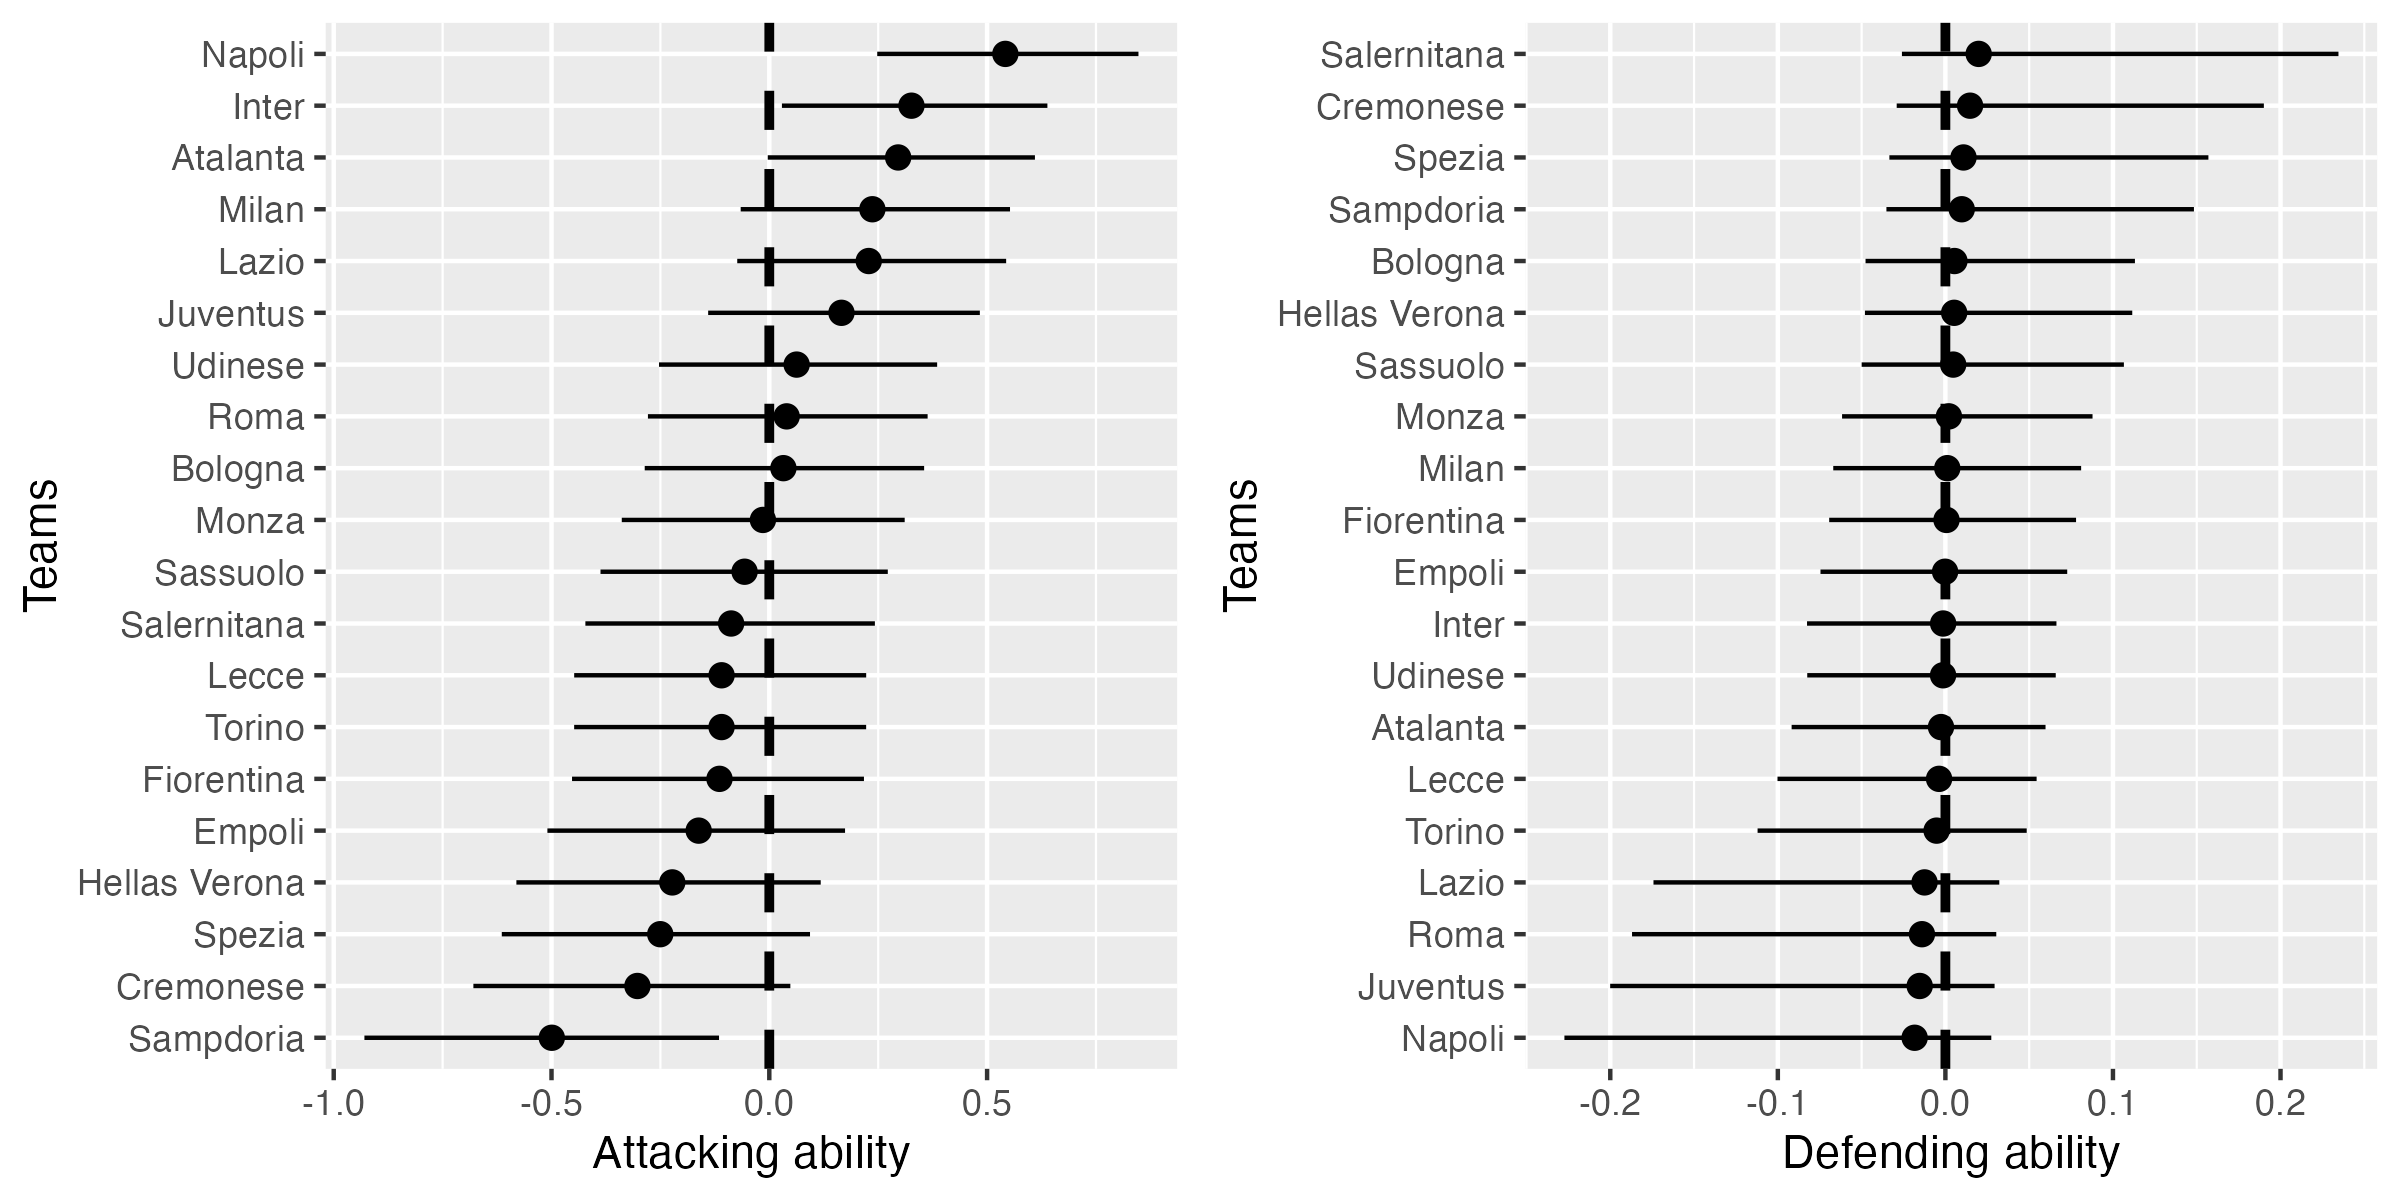
\includegraphics[width=400px]{saattdef} \end{center}

Attack and Defense effects on the same grid give an idea of how teams
proficient specific teams are at both defending and attacking relative
to each other. Consider the case below for La Liga in the 2022/23 season
showing by far how Barcelona and Real Madrid are the most outstanding
teams, followed by a cluster of ``next contenders''; Atletico Madrid,
Real Sociedad, and Athletic Club.

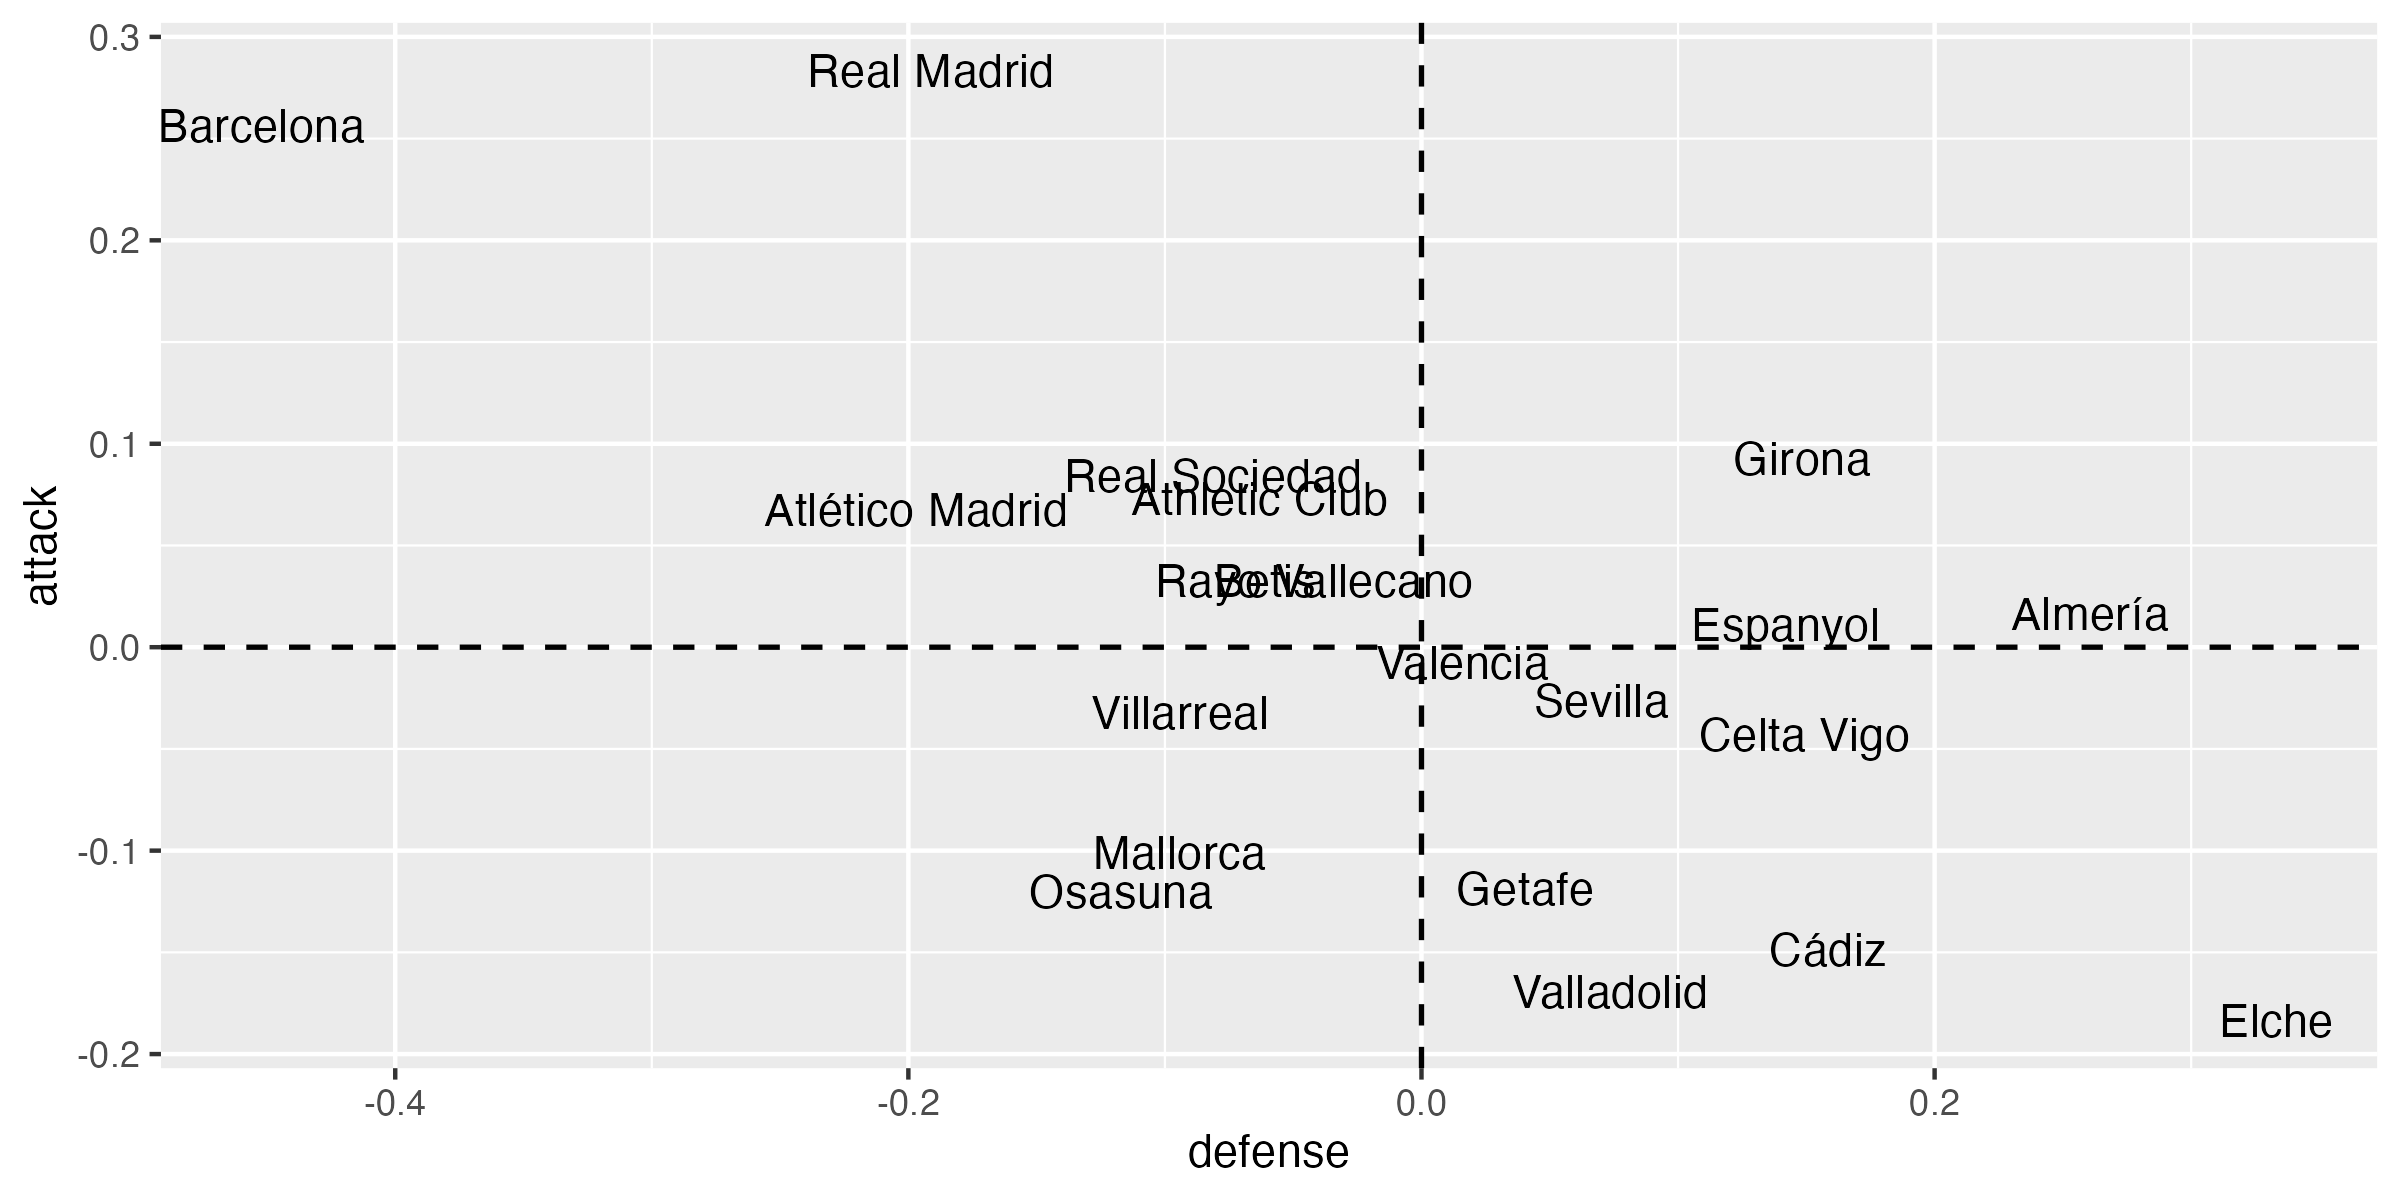
\includegraphics[width=33.33in]{joinedllattdef}

\hypertarget{post-processing}{%
\subsection{Post Processing}\label{post-processing}}

Having run the model through INLA, We are then able to generate the
predictions for goals scored, by simulating from the posterior
distribution for the specific round of matches. Sampling was completed
using R-INLA's method: inla.posterior.sample. Taking the input round
number, data, model, and number of simulations (default 1000) as inputs,
we created a function \texttt{make\_scored()} that will get the index of
corresponding rows. Then the posterior samples of latent variables are
obtained using inla.posterior.sample, say
\(\hat{att_{hi}},\hat{def_{aj}}\) and \(\hat{home}\), storing the
exponentiated posterior sample values. Then we compute the predicted
scoring intensity paramter by each team in the specific round:

\[\hat{\lambda_{ij}} = \exp(\hat{att_{hi}} + \hat{def_{aj}} + \hat{home} + \text{offset})\]
Finally the function generates the predictions for the number of goals
by simulating from a Poisson Distribution using \texttt{rpois()}, with
the predicted scoring intensity parameter:

\[goals_{ij} \sim  \text{Poisson} ( \hat{\lambda_{ij}} )\]

The code used in the modelling process includes utility functions that
manipulate, visualise, and simulat from our dataset to generate
predictions.

** Prediction Processing: * \texttt{datprep()} , preps the data of a
leagueto be used in our \texttt{runINLA()} function. *
\texttt{runINLA()} , runs the INLA model after specifying the formula,
data for given round, posterior family, * \texttt{make\_scored()} ,
Processing function create to predict the number of goals scored by a
team in a given fixture round.

** Visulisation: * \texttt{team\_strength()} , Display Only Attack or
Defence Defence random effects for teams in a league *
\texttt{attack\_defense()} , Display Both Attack and Defence effects on
the same plot, from the INLA model summary * \texttt{outcome\_predict()}
, gives the predicted probabilities of either winning, losing, or
drawing a match. * \texttt{joint\_marginal()} , gives the plot of the
joint posterior probabilities for specified teams Plots the joint
posterior distributions of all the possible scores between two team
given the predicted goals from \texttt{make\_scored()}

** Post-Processing * \texttt{updated\_unplayed()} , extracts the
unplayed fixtures for a given round and inputs the most common result (
i think this should instead be inputting just the sample mean of the
column of goals scored for the team rounded?) *
\texttt{update\_footie()} , updates the premfootie dataset with the goal
predictions * \texttt{var\_updater()} , updates the other variables in
the dataset as a result of the goal predictions * \texttt{roundNinla()}
, streamlines the simulating process, by completing all of the above 3
post-processing for a given round N , e.g round 24

\hypertarget{outcome-predictions}{%
\subsubsection{Outcome predictions:}\label{outcome-predictions}}

Running inla.summary we are able to extract coefficients for estimates
of our models fit. For example in the case of baseline model applied to
Serie A;

\begin{table}

\caption{\label{tab:unnamed-chunk-3}Serie A Fixed Effects; only 2022-2023 Seasons}
\centering
\begin{tabular}[t]{l|r}
\hline
  & mean\\
\hline
(Intercept) & 0.088\\
\hline
Home & 0.213\\
\hline
\end{tabular}
\end{table}

\begin{table}

\caption{\label{tab:unnamed-chunk-3}Hyperparameter Precision in Serie 2022/23 Season}
\centering
\begin{tabular}[t]{l|r}
\hline
  & mean\\
\hline
Precision for factor(Team) & 15.378\\
\hline
Precision for factor(Opponent) & 205.856\\
\hline
\end{tabular}
\end{table}

We see mean values for the intercept and Home fixed effect are 0.088 and
0.213 respectively. Thus the model equation will take the form:
\[\log(\lambda_{ij}) = 0.088 + 0.213{home}_j + {att}_{hi} + {def}_{ai} \]
where

for game g, where: * 0.088 is the intercept * \(0.213home_i\) is the
home advantage efffect for home team in game i, 0.213 increase in the
log of the scoring paramater used in the poisson model predicting goals
scored. * \({att}_{hi}\) is the effect for home team of game i *
\({def}_{ai}\) is the effect for away team of game i

We notice from the model output that the precision for Team factor has a
significantly lower precision than opponent factor, indicating
noticeable variability in the attack effects, while very little hy
variation for defence effects. Thus the effect of an opponent on a teams
goal scoring ability (i.e.~a teams ability to defend against a team) has
less impact than the teams innate attacking ability itself.

\hypertarget{overfitting-concerns---introduction-of-multiple-seasons-data}{%
\subsubsection{Overfitting Concerns - Introduction of Multiple Seasons'
Data}\label{overfitting-concerns---introduction-of-multiple-seasons-data}}

The lack of variability accounted for in the model due to overfitting,
thus th mode may be capturing the noise rather than the underlying
pattern, in this case resulting in the lack of variability in th
Opponent random effect. Thus in order to mitigate this concern we
include the use of multiple seasons data as opposed to using a single
season, that only provides 760 rows of data. With the inclusion of the
2019/20, 2020/21, and 2021/22 along with the 2022/23 seasons, this now
results in dataframes with 3040 rows of data for each league. The
effects of overfitting are also demonstrated in the random effect
quantile plots, particularly for the Opponent (Defence) factor. Consider
the case of the Premier League, where the magnitude of the effects are
considerably small and closely centered around the mean;

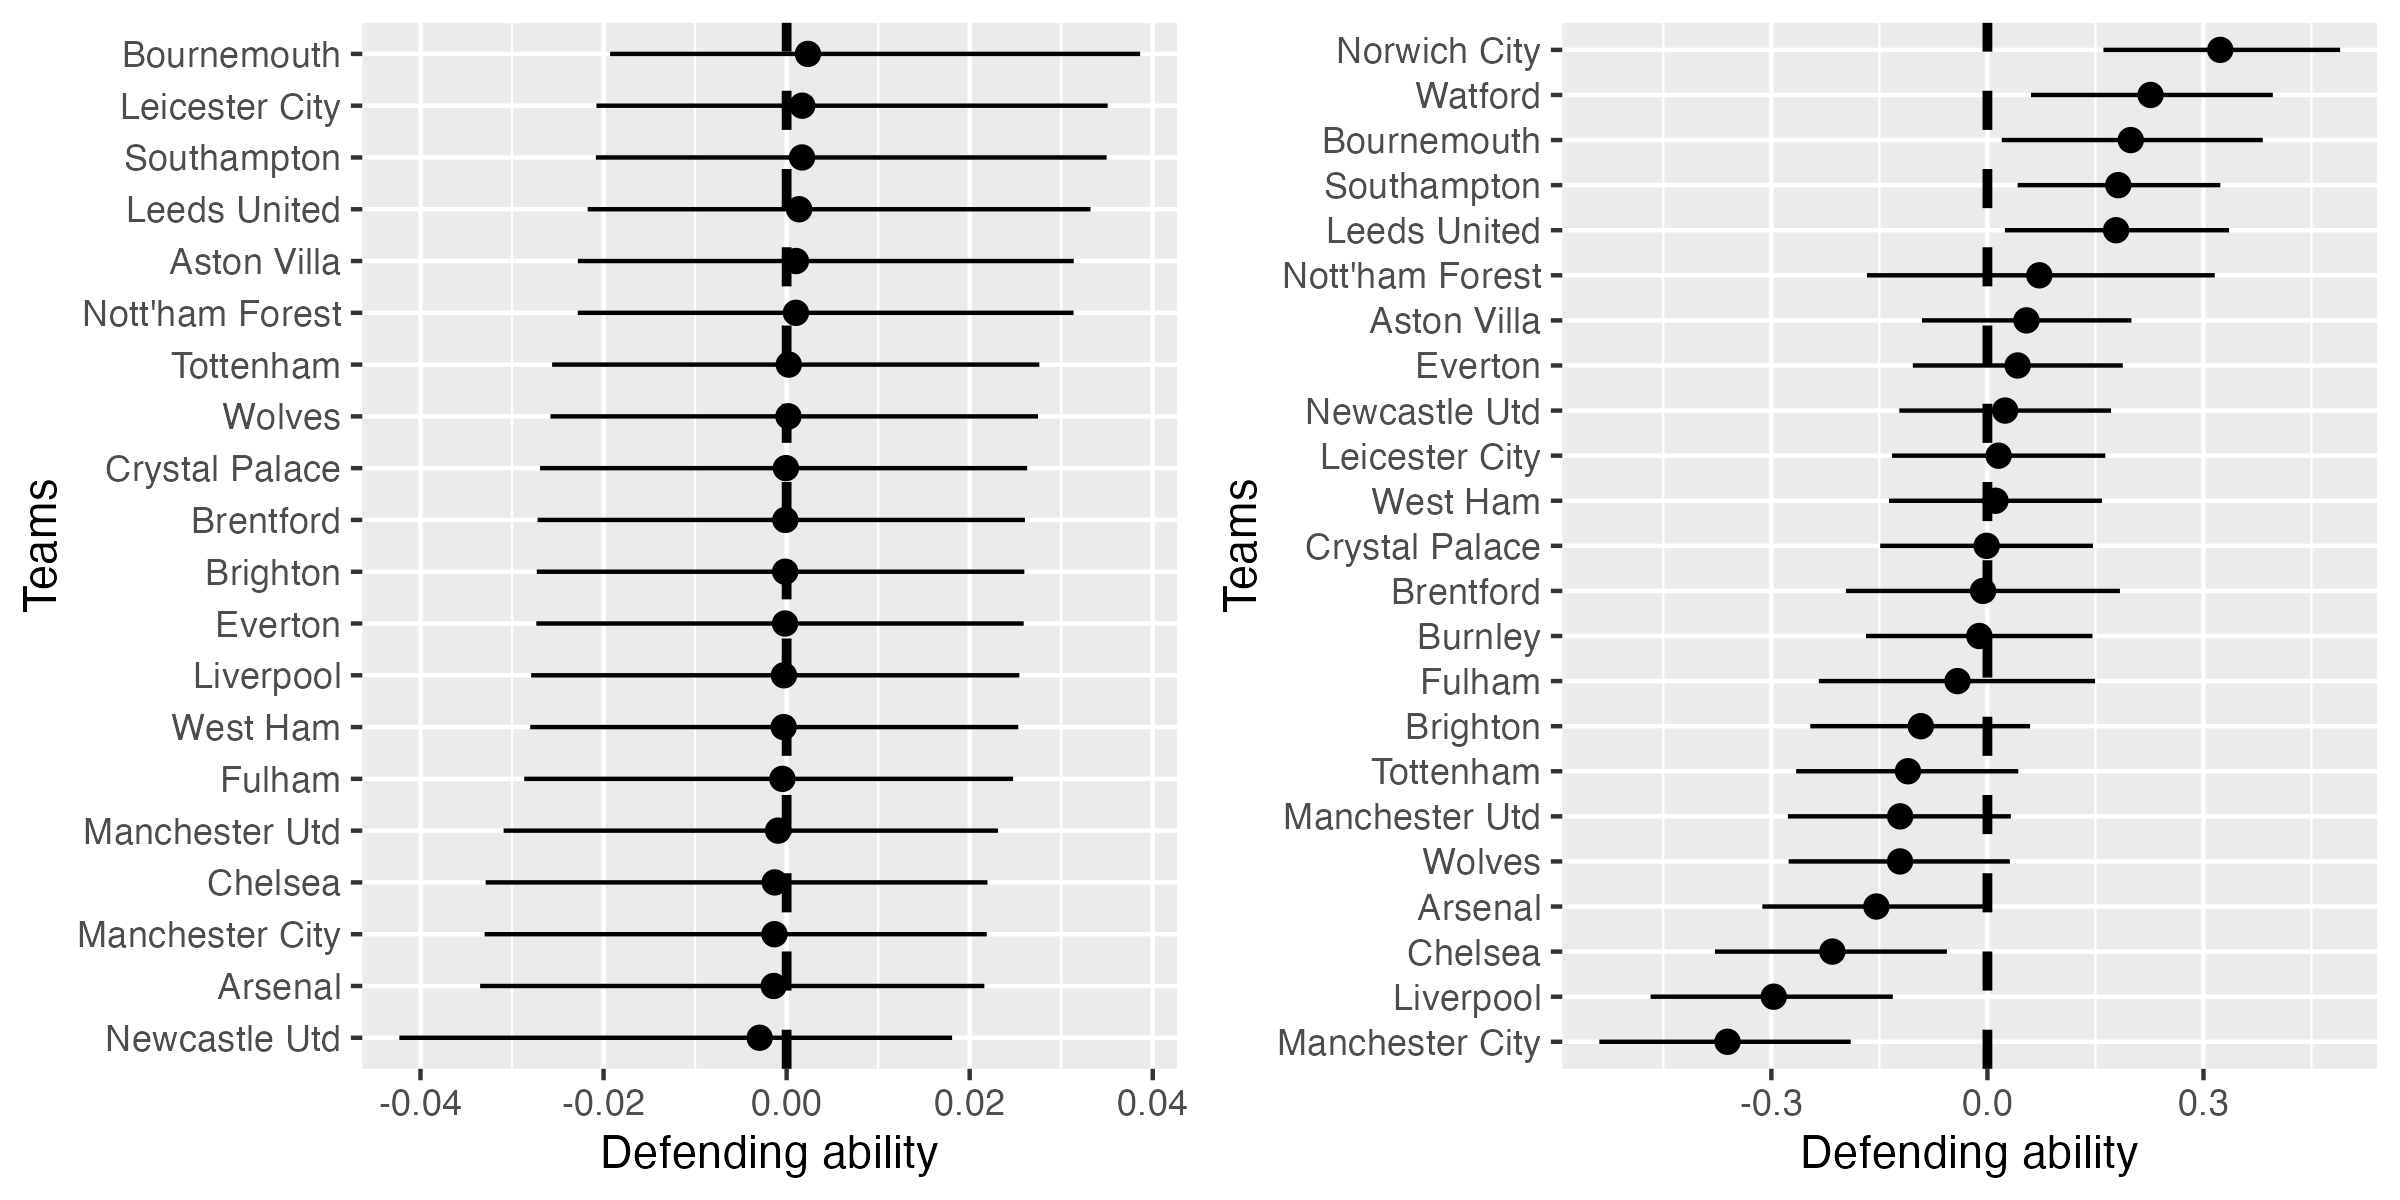
\includegraphics[width=33.33in]{allvssingledefprem} After adding
multiple seasons of data, we see how there is now noticeable variability
in the defence effect for all teams. Thus demonstrated how we have
mitigated the impact of overfitting by adding more data from multiple
seasons. We also see this in the inla.summary output shown below, where
the precision for the model hyperparameters are considerably smaller;
mean 18194.995 when only using 2022/23 compared to 33.254 for 2019-2023
data.

\begin{table}

\caption{\label{tab:unnamed-chunk-5}Hyperparameter Precision using only 2022-2023 Season}
\centering
\begin{tabular}[t]{l|r}
\hline
  & mean\\
\hline
Precision for factor(Team) & 11.605\\
\hline
Precision for factor(Opponent) & 18194.995\\
\hline
\end{tabular}
\end{table}

\begin{table}

\caption{\label{tab:unnamed-chunk-5}Hyperparameter Precision using 2019-2023 Seasons}
\centering
\begin{tabular}[t]{l|r}
\hline
  & mean\\
\hline
Precision for factor(Team) & 12.364\\
\hline
Precision for factor(Opponent) & 33.254\\
\hline
\end{tabular}
\end{table}

\hypertarget{result-generation}{%
\subsection{Result Generation}\label{result-generation}}

Now that we are able to generate predictions using the
inla.posterior.sample method for the number of goals scored for each
team after a given round, we are then able to get predicted match
outcomes for the selected fixtures. In similar research the use of
posterior means or medians is used from both individual team's marginal
distribution, however in our modelling we use the most probable outcome
from the joint posterior predictive distribution in each fixture,
i.e.~the most common row outcome between two teams after each n row
simulations are complete.

For instance, using the baseline model in round 23 of the 2022/23 La
Liga season, in a match between Villarrael and Getafe. We have the
table:

\begin{table}[!h]

\caption{\label{tab:unnamed-chunk-6}Most Probable Outcomes: Villarael v Getafe, Round 23 of La Liga 2022/23}
\centering
\begin{tabular}[t]{r|r|r}
\hline
Villarael & Getafe & prop\\
\hline
1 & 0 & 0.174\\
\hline
1 & 1 & 0.129\\
\hline
0 & 0 & 0.127\\
\hline
2 & 0 & 0.123\\
\hline
0 & 1 & 0.109\\
\hline
2 & 1 & 0.068\\
\hline
\end{tabular}
\end{table}

Here `prop' is the proportion of outcomes with the given result, thus in
this case 17.4\% of outcomes in the match see Villarrael as victors
specifically with a score of 1-0.

We can visually display the joint marginal distribution of goals scored
in this specific match, using our created function:
\texttt{joint\_marginal()}.

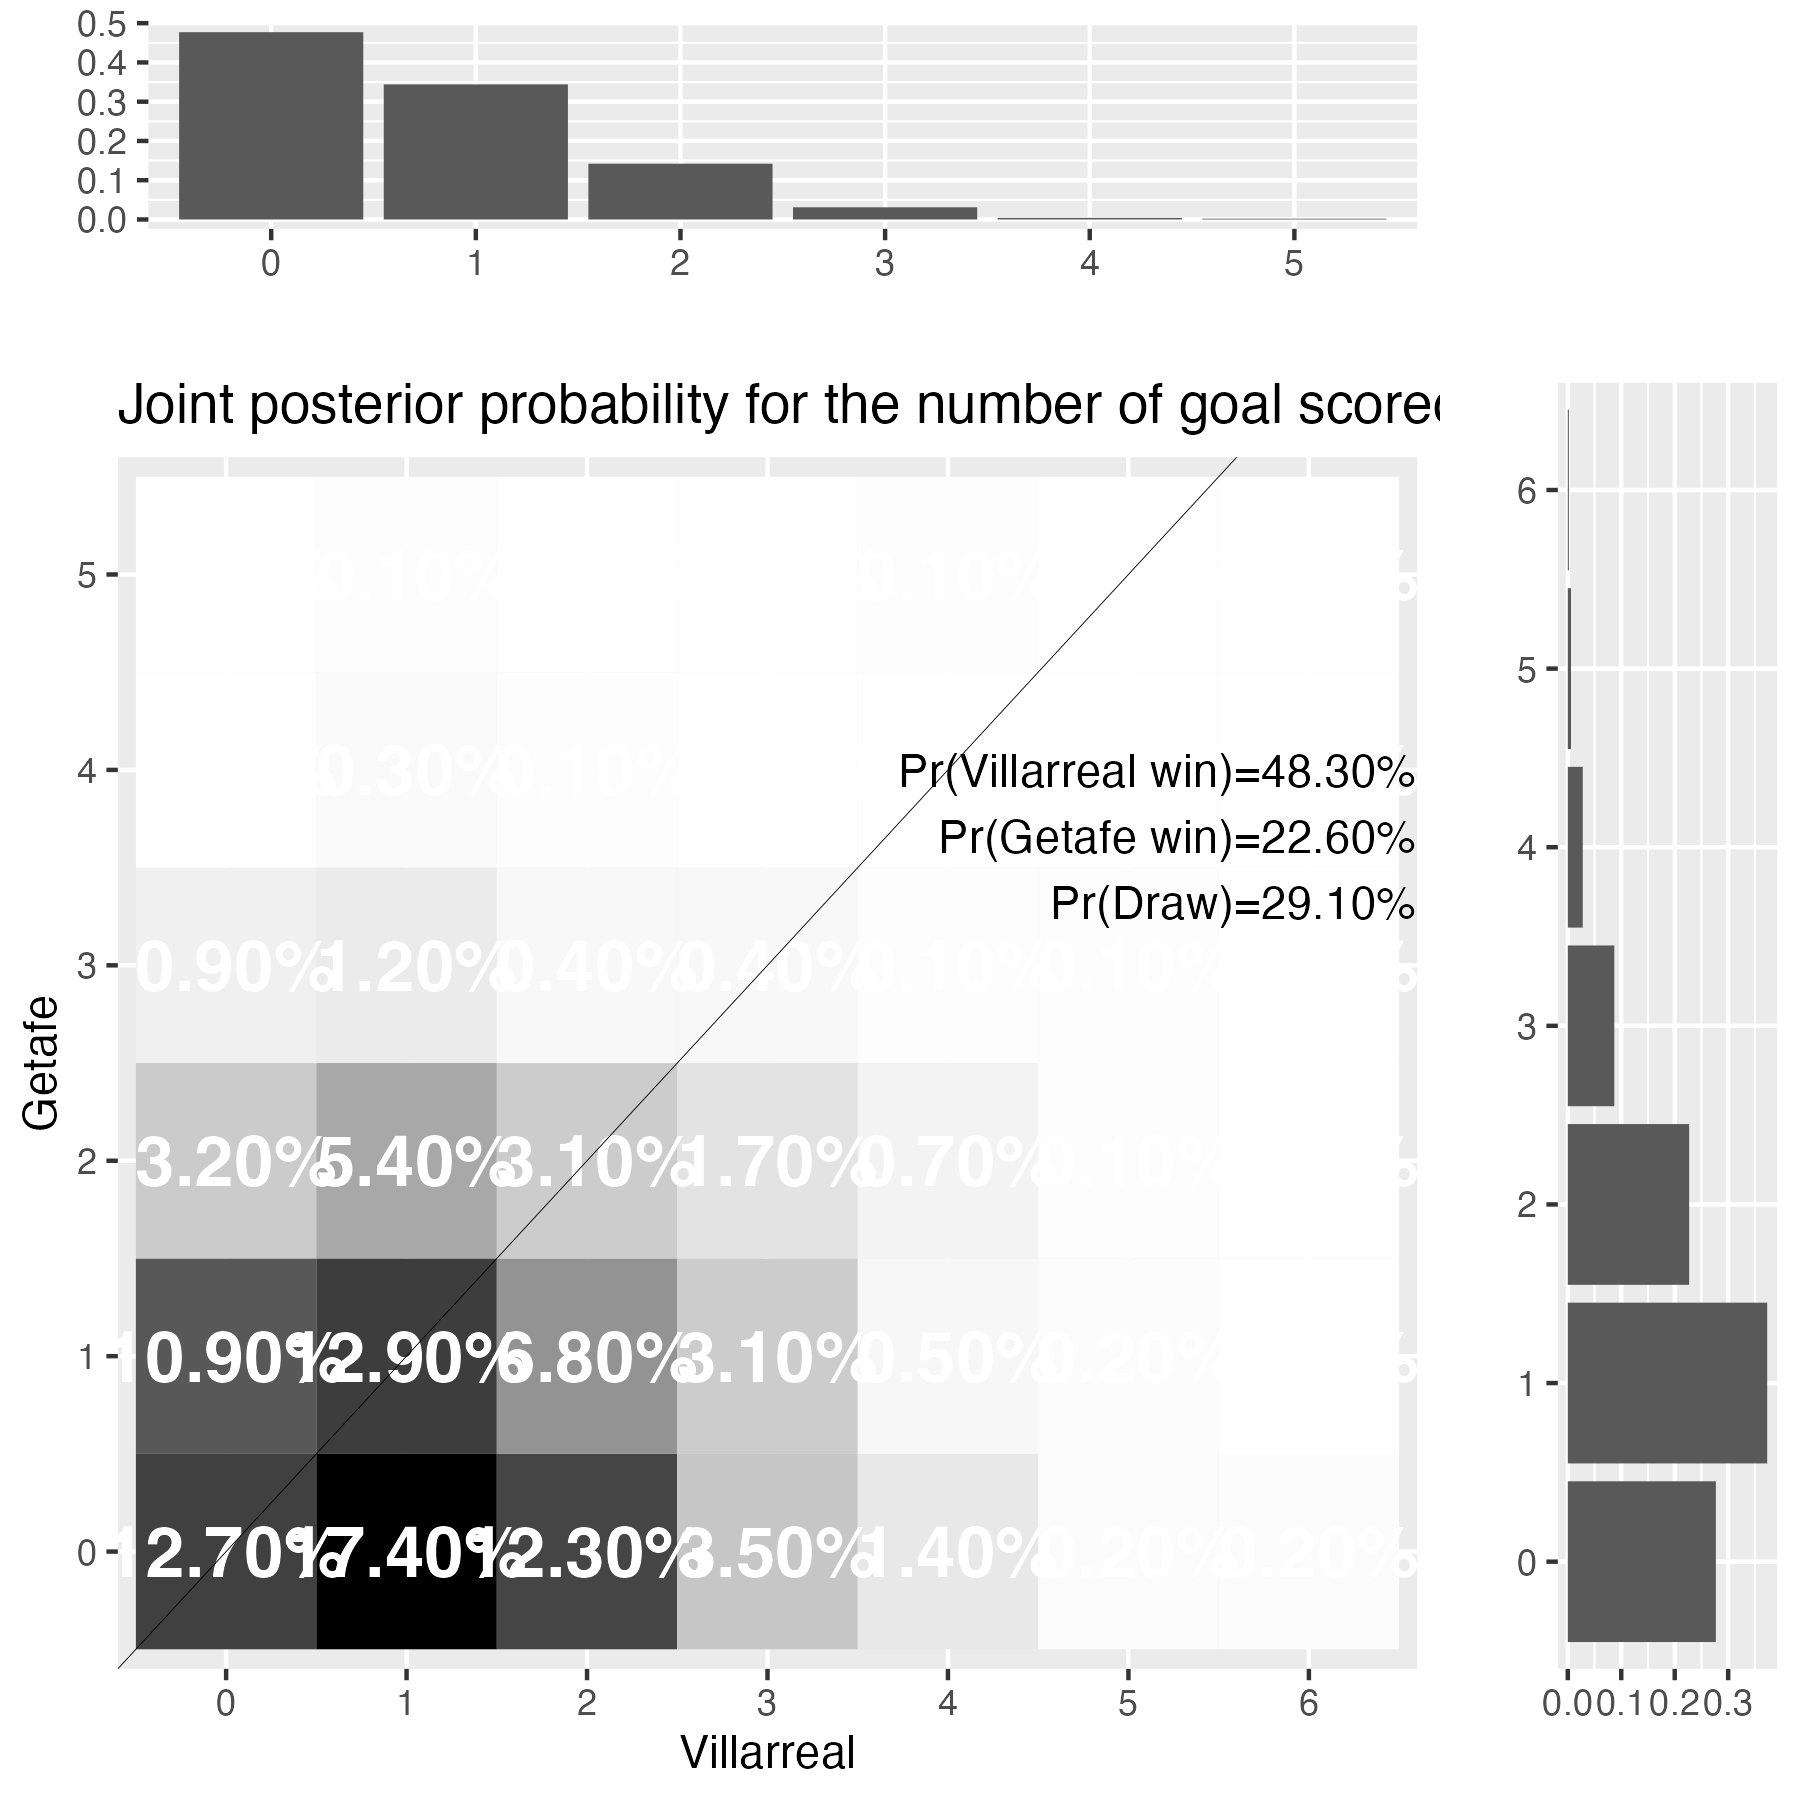
\includegraphics[width=25in]{VillaraelGetafeJM}

We see the probability of every possible outcome from the joint
posterior distribution, along with the overall probability of winning,
drawing, or losing found using our created \texttt{outcome\_predict()}
function. The histograms represents the sampled marginal posterior
distribution for teams individually, with highest density of 0 goal
scored for Getafe (top), and 1 for Villarrael (Right).

After determining the most likely result of relevant `Goal' column, as
well as the associated variables derived from it such as Points , Goal
Difference, Relative Strength etc. Although as before these are not used
in the baseline model.

In the case of Bundesliga, we calculate the cumulative points determined
from goals scored in each game, and derive the league table at the end
of the season: We first show the results when using the Mean of each
teams predicted goals after n simulations, compared to using the joint
predictive posterior distribution. Using means shows Bayern Munich
winning the league, where as the most probable outcome from the joint
distributions leads to Dortmund winning the league

\hypertarget{implementation-of-other-covariates}{%
\subsubsection{Implementation of Other
Covariates}\label{implementation-of-other-covariates}}

We next aim to add covariates to the log linear model estimating the
scoring parameter, which follow the form:

Home Goals:

\[log(\lambda_{1i}) = \beta_0 + \beta_1 home + att_{h_i} + def_{a_i} + \sum^m_j\beta_jz_{i1k}\]
where \(\sum^m_j\beta_jz_{i1k}\) are the added set of covariates with
their effect estimates from the set \(\bar{z}= \{ {z_1,z_2,...,z_m} \}\)
Similarly for Away Goals;

\[log(\lambda_{2i}) = \beta_0 + att_{a_i} + def_{h_i} + \sum^m_j\beta_jz_{i2k}\]

The set of possible covariates that can be part of the set
\(\bar{z}= \{ {z_1,z_2,...,z_m} \}\) are coded as: * Days Since last
Game - \texttt{days\_since\_last} * Relative Strength -
\texttt{rel\_strength} * Goals per game - \texttt{Gpg} * Goals conceded
per game - \texttt{GCpg} * Total Goal Difference-Difference -
\texttt{GDdiff} * Rank Difference - \texttt{diff\_rank} * Form -
\texttt{form}

Note some variable from the dataframe are excluded so to reduce
multicollinearity between variables as they are derived from them, such
as Total Goals Conceded, instead using goals conceded per game as well
as total goal difference. Using this variable we aim to select a set
that provides a better fit for predictions. We next consider compare
different combinations of covariates in finding the best fit through
INLA modelling.

\hypertarget{model-selection}{%
\subsection{Model Selection:}\label{model-selection}}

Typically in INLA and hierarchical modelling (Rue et al.~2009), the use
of Deviance Information Criterion and
Watanabe-Alike-Information-Criterion are use as methods of comparing
models in context. DIC is a model that is analogous to the Akaike
information criterion (AIC) used in estimating prediction error, instead
measuring the trade off between model fit and complexity calculated as
follows: \[ DIC(\lambda) =  D(\bar{\lambda}) + 2p_D \] where
\(D(\bar{\lambda})\) is the deviance at the posterior mean of the
parameters and \(p_D\) is the effective number of parameters.

Similarly the Watanabe-Akaike Information Criterion is a indicator of
singular model performance. As defined by Watanabe himself, (Gelman et
al.~2014) WAIC is the ``negative of the average log pointwise predictive
density and thus is divided by n, and does not have the factor of 2'',
although in INLA is is scaled by factor of 2 for comparability with DIC
and other measures of deviance. DIC makes the assumption that the
posterior is approximately multivariate normal, while WAI can be
numerically calculated without information on the true distribution.
WAIC also an extension of the widely used AIC in the Bayesian context,
and also offers the bonus of no need for effective parameters, again
unlike DIC. Given the added applicability to general BHM methods, the
WAIC is a better indicator of model suitability.

\hypertarget{optimised-model-formulas-for-log-linear-models}{%
\subsection{Optimised Model Formulas for Log Linear
Models}\label{optimised-model-formulas-for-log-linear-models}}

\hypertarget{premier-league}{%
\subsubsection{Premier League}\label{premier-league}}

Below is a table showing the top 10 models with the lowest WAIC,
indicating top 10 most suitable models given the fact that lower WAIC
demonstrates desirable lower deviance. Consider the example below of the
Premier League, where the formula that results in the lowest WAIC
includes added covariates Form, Goals Per Game (Gpc), Goals Conceded Per
Game (GCpg), and Goal Difference-Difference between teams (GDdiff).

\begin{table}[!h]

\caption{\label{tab:unnamed-chunk-8}Top 10 Model Combinations By WAIC: Premier League}
\centering
\resizebox{\linewidth}{!}{
\begin{tabular}[t]{c|c}
\hline
Formula & WAIC\\
\hline
Goal \textasciitilde{} Home + form + Gpg + GCpg + GDdiff + Att + Def & 6642.466\\
\hline
Goal \textasciitilde{} Home + form + days\_since\_last + Gpg + GCpg + GDdiff + Att + Def & 6643.580\\
\hline
Goal \textasciitilde{} Home + rel\_strength + form + Gpg + GCpg + GDdiff + Att + Def & 6643.728\\
\hline
Goal \textasciitilde{} Home + diff\_rank + form + Gpg + GCpg + GDdiff + Att + Def & 6643.918\\
\hline
Goal \textasciitilde{} Home + Gpg + GCpg + GDdiff + Att + Def & 6644.575\\
\hline
Goal \textasciitilde{} Home + rel\_strength + form + days\_since\_last + Gpg + GCpg + GDdiff + Att + Def & 6644.813\\
\hline
Goal \textasciitilde{} Home + rel\_strength + diff\_rank + form + Gpg + GCpg + GDdiff + Att + Def & 6644.870\\
\hline
Goal \textasciitilde{} Home + diff\_rank + form + days\_since\_last + Gpg + GCpg + GDdiff + Att + Def & 6645.032\\
\hline
Goal \textasciitilde{} Home + days\_since\_last + Gpg + GCpg + GDdiff + Att + Def & 6645.622\\
\hline
Goal \textasciitilde{} Home + rel\_strength + Gpg + GCpg + GDdiff + Att + Def & 6645.838\\
\hline
\end{tabular}}
\end{table}

Thus the optimal formula for the Premier League model after this part of
the model building process is of the form:

Home Goals in game i:
\[log(\lambda_{1i}) = \beta_0 +  att_{h_i} + def_{a_i} + \beta_1 Home_j + \beta_2 form + \beta_3 Gpg + \beta_4 GCpg +  \beta_5GDdiff\]
Away Goals in game i:

\[log(\lambda_{2i}) = \beta_0 +  att_{h_i} + def_{a_i} + \beta_1 form + \beta_2 Gpg + \beta_3 GCpg +  \beta_4 GDdiff\]

As for the other domestic leagues, the optimised formulae for the log
linear models are:

\hypertarget{la-liga}{%
\subsubsection{La Liga:}\label{la-liga}}

Home Team:
\[log(\lambda_{1i}) = \beta_0 +  att_{a_i} + def_{h_i} +  \beta_1 Home + \beta_2 Gpg + \beta_3 GCpg + \beta_4 GDdiff\]
Away Team:
\[log(\lambda_{2i}) = \beta_0 +  att_{h_i} + def_{a_i} + \beta_1 Gpg + \beta_2 GCpg +  \beta_3 GDdiff\]

\hypertarget{serie-a}{%
\subsubsection{Serie A:}\label{serie-a}}

Home Team:
\[log(\lambda_{1i}) = \beta_0 +  att_{a_i} + def_{h_i} +  \beta_1 Home + \beta_2 Gpg + \beta_3 GCpg + \beta_4 GDdiff + \beta_5 Form\]
Away Team:
\[log(\lambda_{2i}) = \beta_0 +  att_{h_i} + def_{a_i} + \beta_1 Gpg + \beta_2 GCpg +  \beta_3 GDdiff + \beta_4 form\]

\hypertarget{bundesliga}{%
\subsubsection{Bundesliga:}\label{bundesliga}}

Home Team:
\[log(\lambda_{1i}) = \beta_0 +  att_{a_i} + def_{h_i} +  \beta_1 Home + \beta_2 Gpg + \beta_3 GCpg + \beta_4 GDdiff\]
Away Team:
\[log(\lambda_{2i}) = \beta_0 +  att_{h_i} + def_{a_i} + \beta_1 Gpg + \beta_2 GCpg +  \beta_3 GDdiff\]

\hypertarget{ligue-1}{%
\subsubsection{Ligue 1:}\label{ligue-1}}

Home Team:
\[log(\lambda_{1i}) = \beta_0 +  att_{a_i} + def_{h_i} +  \beta_1 Home + \beta_2 Gpg + \beta_3 GCpg + \beta_4 GDdiff + \beta_5 diffrank\]
Away Team:
\[log(\lambda_{2i}) = \beta_0 +  att_{h_i} + def_{a_i} + \beta_1 Gpg + \beta_2 GCpg +  \beta_3 GDdiff + \beta_4 diffrank\]
\#\# Aditional Covariate Consideration

We also explore the addition of other covariates that may further
improve model performance. First, a time component that aims to address
team's difference in performance over time. This is added to the INLA
model using
\texttt{f(id\_date,model="rw2",replicate=as.numeric(factor(Team)))}. A
Random Walk model of order 2 \texttt{model="rw2"} based on the fixture
date variable representing the time component, is computed separately
for each team \texttt{replicate=as.numeric(factor(Team))}. The effects
from the Random Walk over the course of the dates in our dataset
(between the start of the 2019 season and end of the 2023 season) are
shown in the plot below:

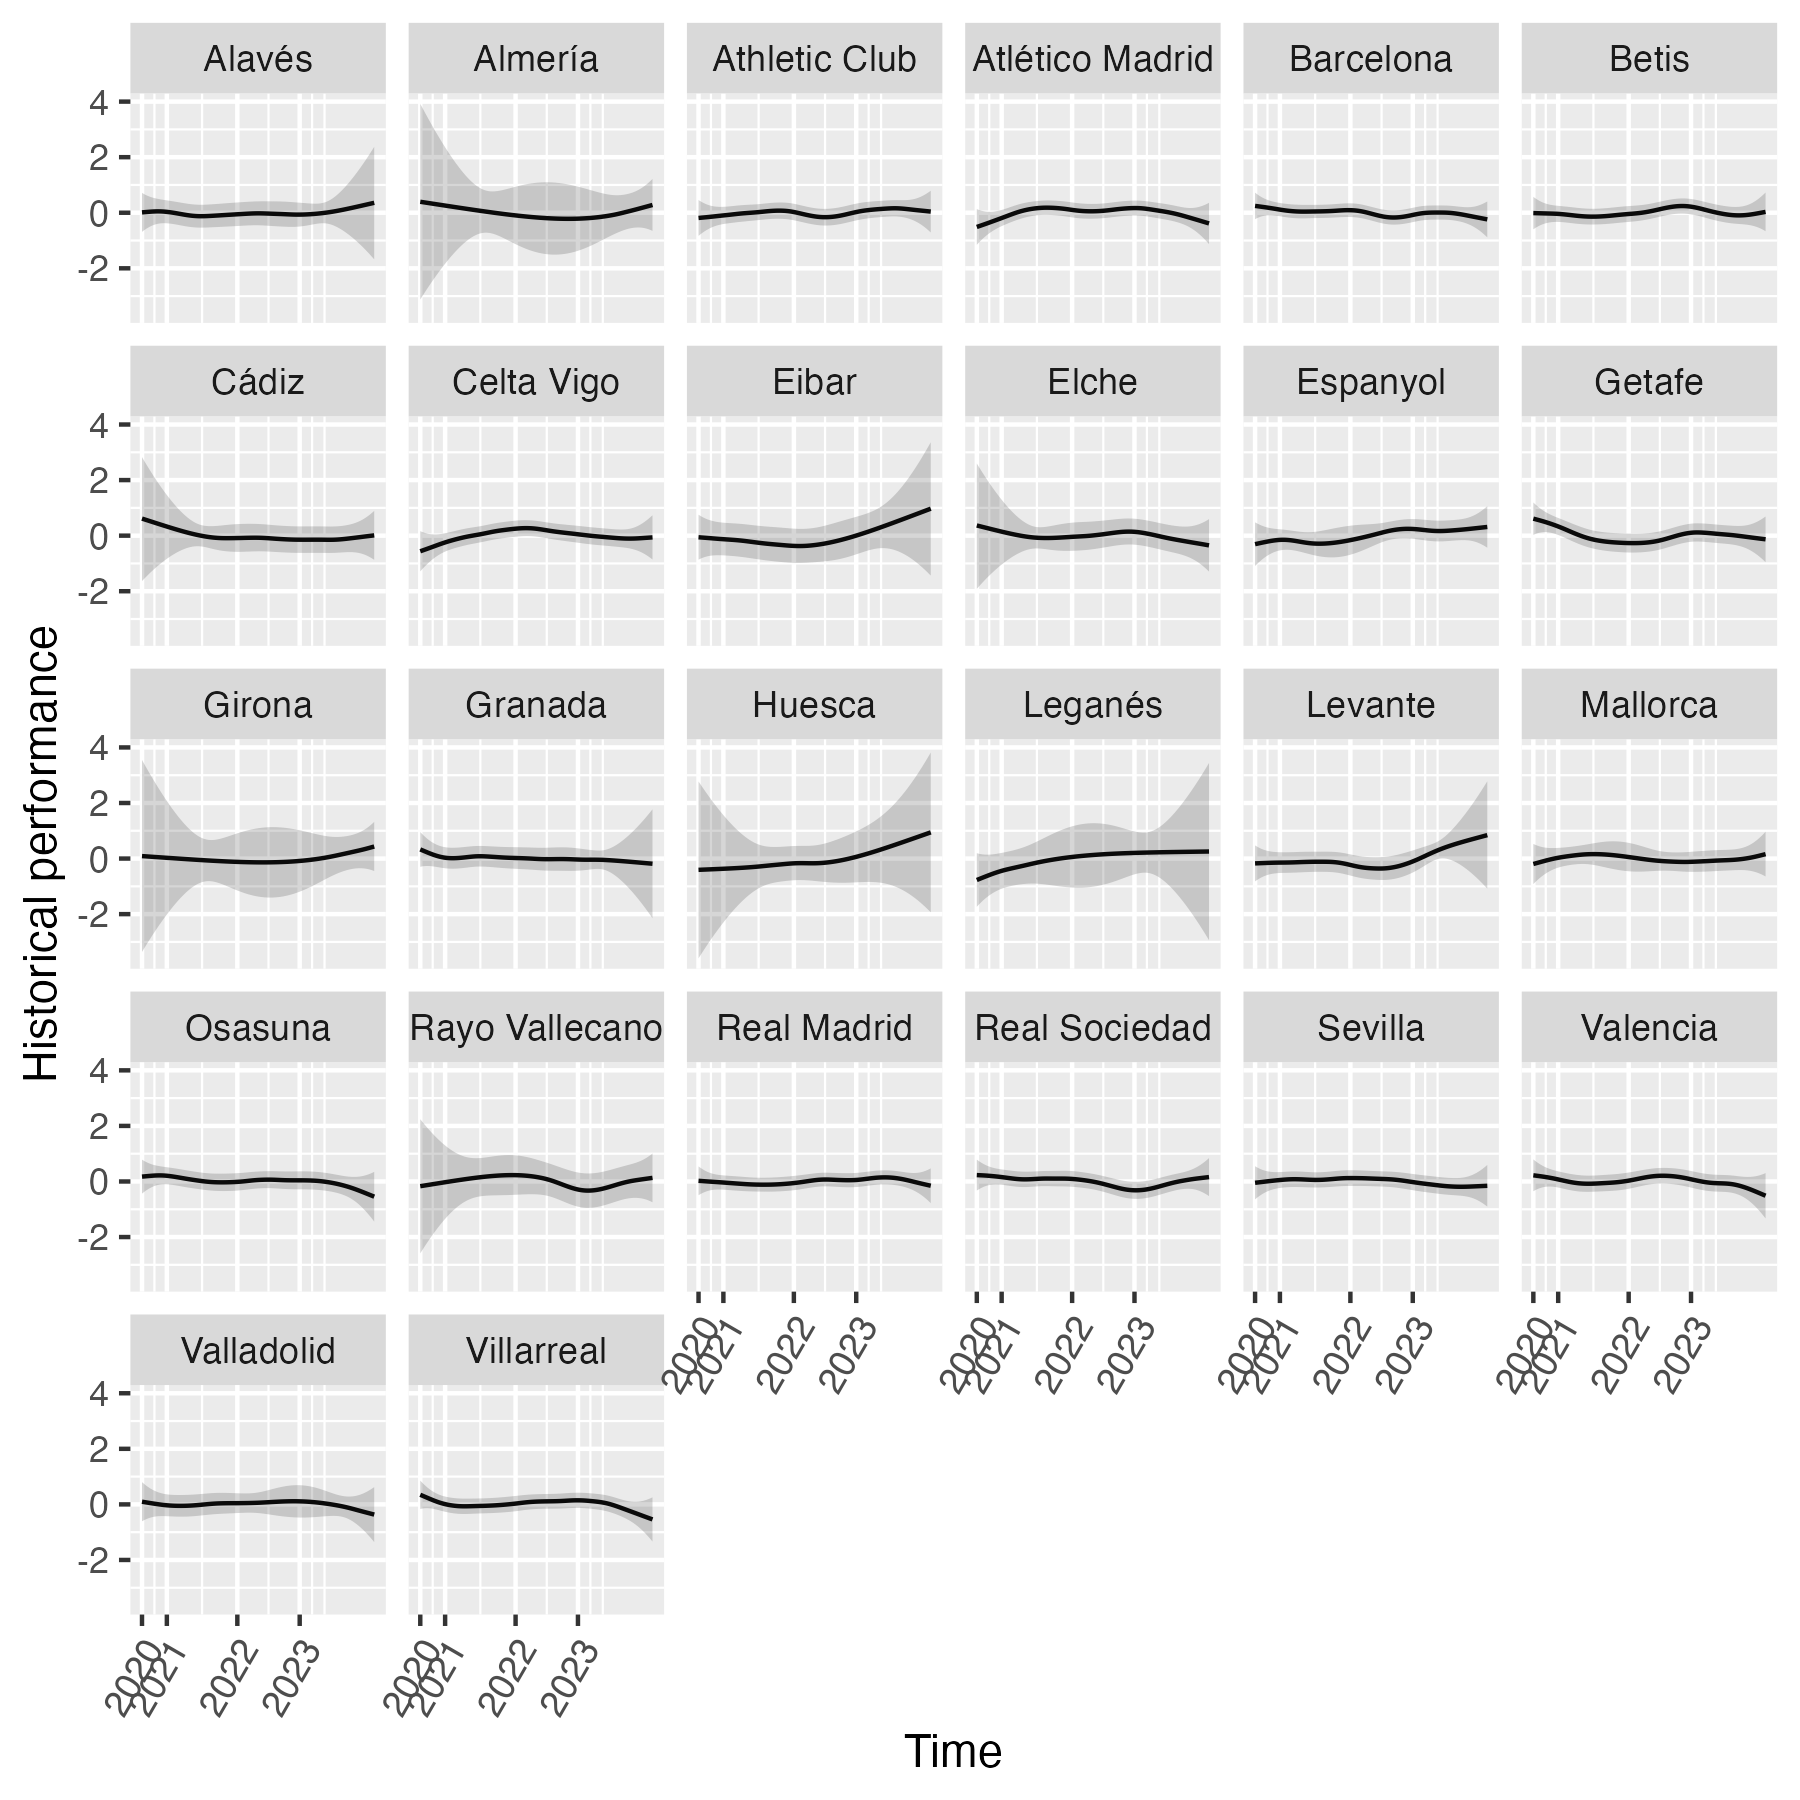
\includegraphics[width=25in]{LaligaTTplot}

Another are of Bayesian Hierarchical Modelling to consider is
overdispersion, a common feature in count data like goals scored in
football. Overdispersion occurs when variance of the observed data is
greater than what would be expected under a simple Poisson distribution,
thus we aim to capture extra variability that may not be accounted for
with other covariates. This is demonstrated in the code by
\texttt{f(num,model="iid")} which adds another random effect to the INLA
model, based on `num' which is the unique identifier of every row in the
data.

However after adding these variables individually and together, they did
not improve model fit by WAIC; adding the random walk time component
increased deviation, while adding the overdispersion parameter neither
improved or negatively impacts WAIC by a noticeable amount. We note the
very high in precision in the model hyperparameters for these added
random effects via the summary output, demonstrating the lack of
variability that is captured by these covariates. Thus we continue
without them.

\hypertarget{model-validation}{%
\subsection{Model Validation}\label{model-validation}}

In model validation we aim to compare the effectiveness of the more
complex `optimised' model, based off WAIC, and the baseline model. This
is executed using all the prior seasons data, with observed data up
until halfway through the 2021/22 season. We then simulate the remainder
of the 2021/22 seasons for each league, and compare with the observed
results of the final league positions for each team. The mean square
error of the optimised and baseline model are compared, and we proceed
to the 2022/23 modelling based on which model has lower MSE. Consider
the case of the Premier League model validation, the table below shows
the predictive performance of the

\begin{table}[!h]

\caption{\label{tab:unnamed-chunk-11}Comparing Baseline and Optimised models Performance vs Obesrved}
\centering
\resizebox{\linewidth}{!}{
\begin{tabular}[t]{l|r|r|r|r|r}
\hline
Team & Observed\_Points & Baseline\_Points & Baseline\_Difference & Optimized\_Points & Optimized\_Difference\\
\hline
Arsenal & 69 & 56 & 13 & 56 & 13\\
\hline
Aston Villa & 45 & 61 & 16 & 47 & 2\\
\hline
Brentford & 46 & 35 & 11 & 37 & 9\\
\hline
Brighton & 51 & 36 & 15 & 44 & 7\\
\hline
Burnley & 35 & 33 & 2 & 35 & 0\\
\hline
Chelsea & 74 & 67 & 7 & 61 & 13\\
\hline
Crystal Palace & 48 & 57 & 9 & 42 & 6\\
\hline
Everton & 39 & 37 & 2 & 39 & 0\\
\hline
Leeds United & 38 & 44 & 6 & 36 & 2\\
\hline
Leicester City & 52 & 51 & 1 & 47 & 5\\
\hline
Liverpool & 92 & 65 & 27 & 68 & 24\\
\hline
Manchester City & 93 & 86 & 7 & 74 & 19\\
\hline
Manchester Utd & 58 & 60 & 2 & 56 & 2\\
\hline
Newcastle Utd & 49 & 35 & 14 & 35 & 14\\
\hline
Norwich City & 22 & 34 & 12 & 31 & 9\\
\hline
Southampton & 40 & 41 & 1 & 42 & 2\\
\hline
Tottenham & 71 & 61 & 10 & 56 & 15\\
\hline
Watford & 23 & 32 & 9 & 28 & 5\\
\hline
West Ham & 56 & 62 & 6 & 54 & 2\\
\hline
Wolves & 51 & 56 & 5 & 51 & 0\\
\hline
\end{tabular}}
\end{table}

Using the figures above we are able to calculated the mean squared error
for the baseline model and optimised models respectively; 115.55, 100.65
thus demonstrating we have achieved better performance using the
optimised formula in the log linear model for the scoring parameters.
The improved performance is consistent with results of Bundesliga, Serie
A, and La Liga, all of which had lower MSE than their baseline models.
However in the case of Ligue 1, as the baseline model achieves lower
MSE. This may be due to the reduce number of data points used in
modelling. In the 2019/20 seasont the COVID-19 Pandemic resulted in the
distruption of football scheduling in the domestic leagues, and while
the other four returned to action, Ligue 1 ended halfway through. Thus
when modelling using data from 2019-2023, there are missing observations
that were removed for the French league. This means that the baseline
model, which is stronger at identifying variability in team attack and
defence random effects, may better fit the league with fewer data
available, since the otimised model may overfit the data.

We thus model the 2022/23 seasons using the optimised log linear models
for the Premier League, Bundesliga, Serie A, and La liga, whilst using
the baseline model for Ligue 1.

\hypertarget{final-predictions}{%
\subsection{Final Predictions}\label{final-predictions}}

Now that we have final models to predict performances in the European
domestic leagues, we return to the original questions; How will the
teams perform in the 2022/2023 season? How will the results fair with
the removal of the Super League Teams?

\hypertarget{predicting-with-super-league-teams}{%
\subsubsection{Predicting with Super League
Teams}\label{predicting-with-super-league-teams}}

\hypertarget{premier-league-1}{%
\paragraph{Premier League}\label{premier-league-1}}

\hypertarget{la-liga-1}{%
\paragraph{La Liga}\label{la-liga-1}}

\hypertarget{bundesliga-1}{%
\paragraph{Bundesliga}\label{bundesliga-1}}

\hypertarget{serie-a-1}{%
\paragraph{Serie A}\label{serie-a-1}}

\hypertarget{ligue-1-1}{%
\paragraph{Ligue 1}\label{ligue-1-1}}

\hypertarget{predicting-without-super-league-teams}{%
\subsubsection{Predicting Without Super League
Teams}\label{predicting-without-super-league-teams}}

\hypertarget{premier-league-2}{%
\paragraph{Premier League}\label{premier-league-2}}

\hypertarget{la-liga-2}{%
\paragraph{La Liga}\label{la-liga-2}}

\hypertarget{bundesliga-2}{%
\paragraph{Bundesliga}\label{bundesliga-2}}

\hypertarget{serie-a-2}{%
\paragraph{Serie A}\label{serie-a-2}}

\hypertarget{ligue-1-2}{%
\paragraph{Ligue 1}\label{ligue-1-2}}

\hypertarget{discussion-only-sumarries-at-the-moment}{%
\section{Discussion: (ONLY SUMARRIES AT THE
MOMENT)}\label{discussion-only-sumarries-at-the-moment}}

\hypertarget{conclusions}{%
\subsection{Conclusions}\label{conclusions}}

\begin{itemize}
\tightlist
\item
  talk about what we foud in our results compare the withsuperleague to
  withoutsuperleague preditions,
\item
  what are the supposed effect of these predictions? the significance?
\end{itemize}

\hypertarget{limitations}{%
\subsection{Limitations}\label{limitations}}

\begin{itemize}
\item
  A common probablem of the Bayesian Hierarchical model is overshrinkage
  where extreme outcomes, like a team scoring 8 goals, are instead
  pulled towards the grand mean. We notice this in the use of
\item
  Can improve performance using more data
\item
  Lack of Covariates
\end{itemize}

\hypertarget{future-work}{%
\subsection{Future Work}\label{future-work}}

\begin{itemize}
\item
  3 Tier Hierarchical Model
\item
  Machine Learning Techniques?
\item
  add more complex covariates ? player specific level perhaps?
\end{itemize}

etc.

References: (still draft)

\url{https://www.theguardian.com/football/2021/apr/20/uk-government-may-legislate-to-stop-european-super-league-says-minister}

{[}\url{https://www.statista.com/statistics/1230111/european-super-league-sponsorship-revenue/\#}:\textasciitilde:text=Early\%20reports\%20suggested\%20that\%20media,euros\%20annually\%20from\%20these\%20deals{]}

Maher, M. J. (1982). Modelling association football scores. Statistica
Neerlandica, 36(3), 109-118.

Rue, H., \& Salvesen, Ø. (2000). Prediction and Retrospective Analysis
of Soccer Matches in a League. Journal of the Royal Statistical Society.
Series D (The Statistician), 49(3), 399--418.
\url{http://www.jstor.org/stable/2681065}

Godin, F., Zuallaert, J., Vandersmissen, B., De Neve, W., \& Van de
Walle, R. (2014, June). Beating the bookmakers: leveraging statistics
and Twitter microposts for predicting soccer results. In KDD Workshop on
large-scale sports analytics (pp.~2-14). New York, NY, USA: ACM.

Hubáček, O., Šourek, G., \& Železný, F. (2019). Learning to predict
soccer results from relational data with gradient boosted trees. Machine
Learning, 108, 29-47.

Santos-Fernandez, E., Wu, P., \& Mengersen, K. L. (2019). Bayesian
statistics meets sports: a comprehensive review. Journal of Quantitative
Analysis in Sports, 15(4), 289-312.

Schauberger, G., \& Groll, A. (2018). Predicting matches in
international football tournaments with random forests. Statistical
Modelling, 18(5-6), 460-

Hilbe, J. M., De Souza, R. S., \& Ishida, E. E. (2017). Bayesian models
for astrophysical data: using R, JAGS, Python, and Stan. Cambridge
University Press.

Congdon, P.D. (2019). Bayesian Hierarchical Models: With Applications
Using R, Second Edition (2nd ed.). Chapman and Hall/CRC.
\url{https://doi.org/10.1201/9780429113352}

H. Rue, S. Martino, and N. Chopin. Approximate Bayesian inference for
latent Gaussian models using integrated nested Laplace approximations
(with discussion). Journal of the Royal Statistical Society, Series B,
71(2):319, p392, 2009.

Gelman, A., Hwang, J. \& Vehtari, A. Understanding predictive
information criteria for Bayesian models. Stat Comput 24, 997--1016
(2014). \url{https://doi.org/10.1007/s11222-013-9416-2}

\end{document}
